\chapter{The physical linguistics program}

The o/el model is a conceptual framework in the program of \textit{physical linguistics}. The physical linguistics “program” is a set of concepts, values, and methods for the scientific study of language. There are three reasons for describing the program as \textit{physical}: 

  First, linguistic phenomena are understood to arise from nothing more or less than physical systems. This entails a commitment to a worldview in which a model of any relatively macro-scale phenomena should be derivable from models of relatively micro-scale phenomena, regardless of the particular scale on which the phenomena are modelled. Models of language change should be derived from models of language variation in social networks of individuals, models of variation in social networks should be derived from models of individual linguistic behavior, models of individual behavior should derived from models of cognitive systems, models of cognitive systems should be derived from models of neural systems, and so on. Because of the emphasis on relating systems whose dynamics must be characterized on different scales, attention to spatial and temporal scale is crucial in any analysis. The program is reductionist and physicalist: no hidden mind-body dualism is allowed (e.g. a narrow language faculty independent of a sensorimotor interface). In practice, deduction of macro phenomena from micro models is very difficult, and so far the o/el framework falls far short of providing anything more than suggested approaches to such deductions. To a large extent the shortfall is due to lack of knowledge regarding the microscale systems, i.e. neural populations, as well as difficulty in implementing sufficiently realistic models. Derivation of the macro from the micro is a goal, but not a prerequisite to macro-scale theory development.

  Second, the program is \textit{physical} because models of “cognitive” systems are analogized to models of “physical” ones, or understood metaphorically as such. Because cognitive systems \textit{are} physical (see above), these are not really analogies. Cognitive systems are expected to exhibit the same spatial/temporal patterns as those which arise in “non-cognitive” physical systems. The oscillators/energy levels framework is just one example of this: we used concepts of oscillation and energy, which describe many physical systems, as metaphors for conceptualizing cognitive ones. No new concepts must be invented in order to develop a useful understanding of language; instead, already existing concepts can be repurposed to understand the complex patterns of language. The complexity is due to the fact that the relevant systems are most usefully described on a wide range of spatial and temporal scales. There are many other physical analogies/metaphors which one might use to construct an understanding of language; the modus operandi of the program is the exploration of these metaphors.

  Third, the physical program promotes the use of concepts and analytic tools from the physical sciences. Among these two stand out as very useful. One is the method of coarse-graining, in which variables describing the microscale system are integrated over a range of spatial and temporal scales. This procedure provides a basis for drawing inferences regarding relatively macroscopic patterns from a relatively microscopic ones; it also provides us flexibility in the construction of macroscopic systems. The other useful method is systems-surroundings partitioning. Analyses in the o/el framework rely heavily on this partitioning, which can be viewed as a strategy for managing ignorance. We elaborate on these tools further in this chapter.

\section{Physical and computational approaches to studying complex systems}

To contextualize the physical linguistics program and motivate the rhetorical stance of this chapter, we consider two approaches to the study of complex systems. One is the program of synergetics developed by the German physicist Hermann Haken \citep{Haken1973,Haken1983b,Haken1983a}, which deals with multiscale, self-organized systems from a physical perspective. Synergetics has been influential in the development of the o/el framework. The other is the notion of levels of analysis, developed by the neuroscientist David Marr \citep{MarrPoggio1977,Marr1982}. The Marrian approach, while sometimes useful, has been frequently misinterpreted and misapplied to rationalize willful ignorance regarding the microscopic origins of macroscopic phenomena. A close reading of Marr reveals a tension between focusing on the “levels” of analysis and focusing on the interrelations of levels as well as a comprehensive understanding across levels.

\subsection{Synergetics: a physical approach}

The physical linguistics program has in many ways been inspired by the program of synergetics, which was developed by the German physicist Hermann Haken \citep{Haken1973,Haken1983b,Haken1983a}. Synergetics incorporates a vocabulary and mathematical toolkit for modeling the self-organized formation of macroscopic patterns which arise from the interactions of many microscopic subsystems. As \citet{Haken1973} puts it:

\begin{quote}
    Very often the properties of the large systems cannot be explained by a mere random superposition of the actions of the subsystems. Quite on the contrary the subsystems behave in a well organized manner, so that the total system is in an ordered state or shows actions which one might even call purposeful. Furthermore one often observes more or less abrupt changes between disorder and order or transitions between different states of order. Thus the question arises, who are the mysterious demons who tell the subsystems in which way to behave so to create order, or, in a more scientific language, which are the principles by which order is created. (1973: 9)
\end{quote}

A key aspect of the synergetic approach is the concept of an \textit{order parameter}, which according to Haken has two functions. On one hand, the order parameter is a variable that describes order in the system; on the other hand, it “gives orders” \citep[10]{Haken1973} to the subsystems, i.e. influences their states. Haken presents ferromagnets as a prototypical example of a physical system which can be readily conceptualized along these lines. The ferromagnet (i.e. the macroscale system) consists of many individual atoms (the microscale subsystems), each of which has a spin that is either (+) or (-). The spins of these individual atoms are globally aligned when the magnet is below a critical temperature, but lose the global alignment when above the critical temperature. Hence there is a transition from a disordered state to an ordered state as temperature is decreased. The alignment of the spins results from Coulomb force interactions between individual atoms, but is counteracted by random fluctuations that depend on temperature. 

The usefulness of the order parameter—here the mean field of the magnet, an average over the states of the individual atoms—is that it allows for a lower-dimensional description of the system, in contrast to the high-dimensional description that would make reference to the spins of each of the atoms in the magnet. Regarding the second function of the order parameter, the mean field can be conceptualized metaphorically as exerting a “force” on the subsystems. Haken furthermore describes the order parameter and the subsystems as a hierarchical system, in which there exists a “hierarchy of time constants”: the subsystem state dynamics have a much smaller timescale than the dynamics of the order parameter, and changes in their states respond rapidly to variation in the order parameter. 

  Other examples in different domains can be understood in the same framework. In chemical solutions, densities of reactants are the order parameters which describe the macroscopic state of the system, and individual molecules are the subsystems. In a neural network, integrated spiking rate of the network is an order parameter, and individual neurons are subsystems. In ecological systems, numbers of animals are order parameters, and individual animals are subsystems. One point of interest is that when two or more order parameters in a system interact—e.g. the numbers of predators and prey, or the densities of two different types of reactants—a temporal oscillation can arise. Another is that the order parameter can reflect instabilities which induce symmetry breaking: the system is driven to one particular steady state out of a set of possible steady states. 

The relevance of the concepts of instability and symmetry breaking to cognition and behavior are elaborated clearly and thoroughly in \citet{Kelso1997}, and a substantial program of investigation of perception and motor control has been developed along those lines (cf. \citet{Kelso1997} and references therein). One classic example is the Haken-Kelso-Bunz model of bimanual coordination \citep{HakenEtAl1985,SchonerKelso1988}). It had been observed that as rate is increased in a bimanual finger wagging task, an anti-phase pattern of coordination transitions to an in-phase pattern \citep{KelsoEtAl1981}. This transition is represented in {\figref{fig:8:1}}(A), where the positions of each finger over time are plotted as wagging rate (ω) increases. The positions of the fingers can be associated with phase angles (θ\textsubscript{L}, θ\textsubscript{R}), and the relative phase ϕ = θ\textsubscript{L} – θ\textsubscript{R} is considered an order parameter of the system. Note that a description of the system in terms of the 1-dimensional order parameter is simpler than a description that involves a phase angle parameter for each finger. The key phenomenon is that ϕ transitions from a value that is approximately ±π (the anti-phase mode) to 0 (the in-phase mode) at a critical movement frequency, as shown in {\figref{fig:8:1}}(B). Moreover, when the wagging is begun in an in-phase pattern, the reverse transition to an anti-phase pattern does not occur.

  
\begin{figure}
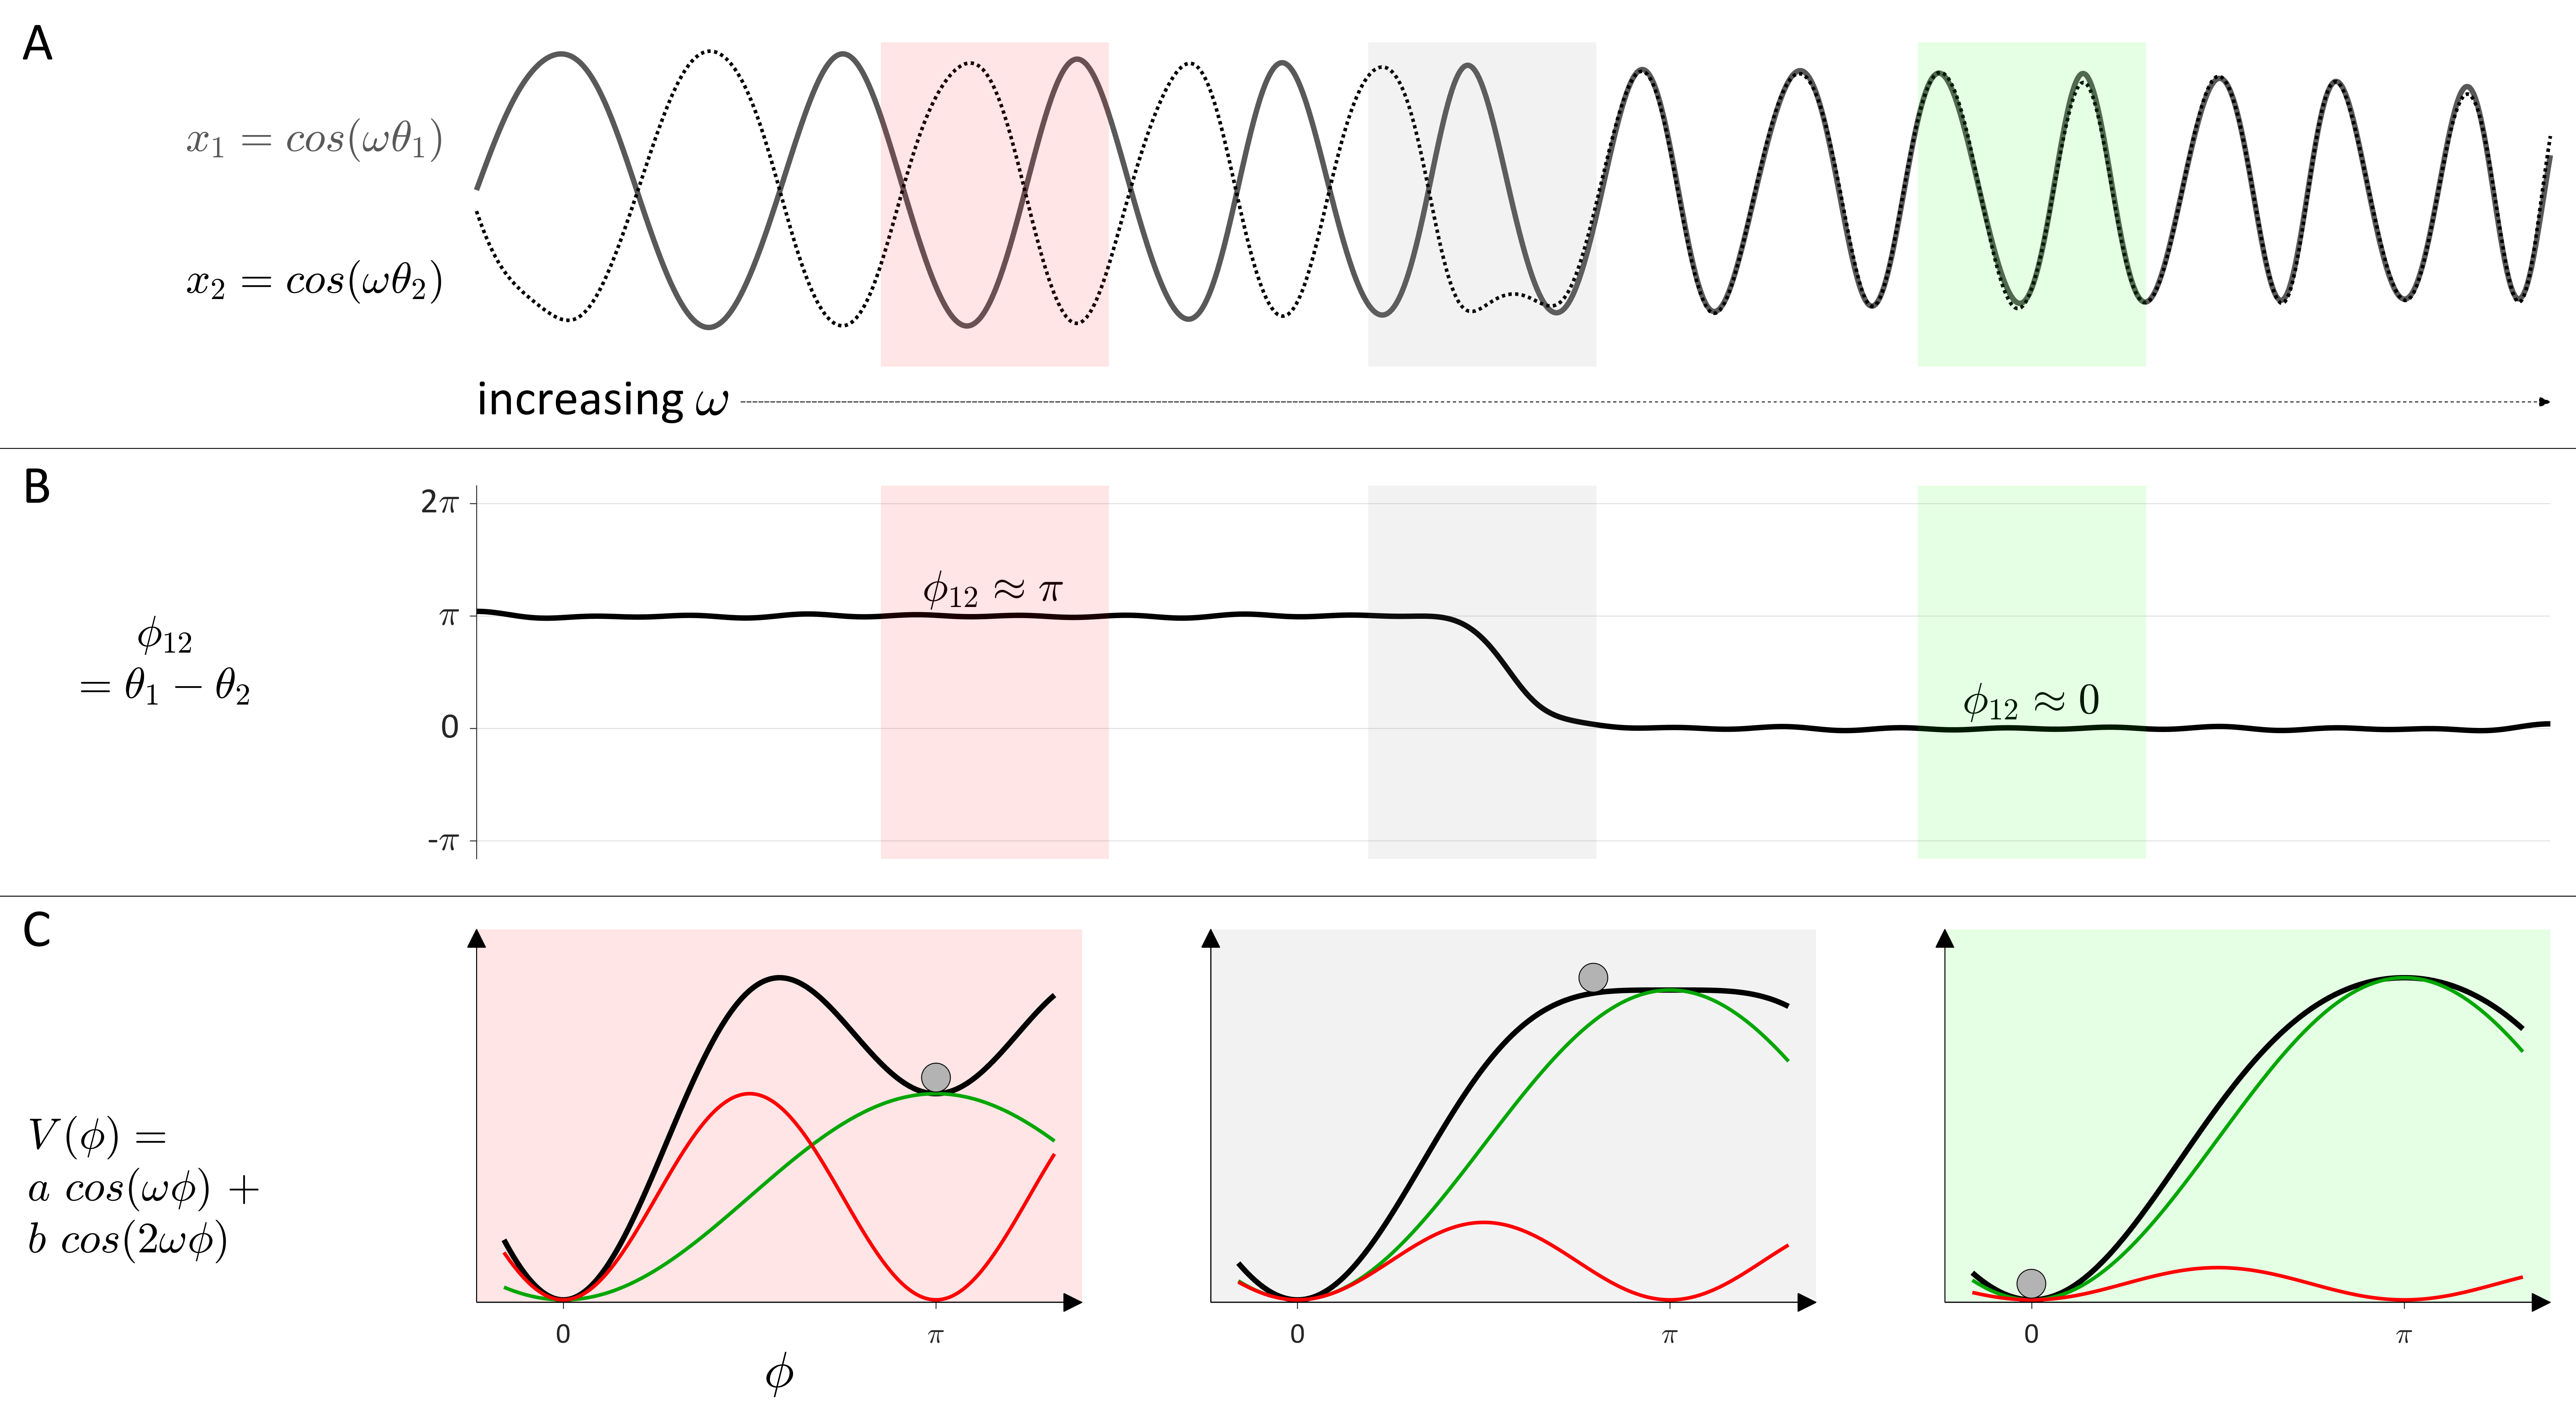
\includegraphics[width=\textwidth]{figures/Tilsen-img167.png}
\caption{Haken-Kelso-Bunz model of anti-phase to in-phase transition in finger wagging.}
\label{fig:8:1}
\end{figure}
 

  The \citet{HakenEtAl1985} model posits that there is a potential function V(ϕ) governing the dynamics of the order parameter ϕ, and that this potential function consists of two components, which are harmonically related cosine functions. The first component has minima at integer multiples of ±2π and the second component has minima at integer multiples of ±π. The authors proposed that at slow rates, the relative amplitude of the second component to the first (b/a) is large and thus the anti-phase mode of coordination is stable, corresponding to the presence of minima at integer multiples of ±π in the potential function, shown in the leftmost panel of {\figref{fig:8:1}}(C). At higher rates, the relative amplitude of the second component decreases and the anti-phase mode of coordination becomes unstable, as shown in the middle panel of (C). This induces a phase transition to the in-phase mode, as shown in the rightmost panel of (C). The equations of motion in the model include terms for both intrinsic oscillation of the effectors and for coupling between effectors, mediated via the potential function. The model has been extended to include coupling between systems with oscillations of different frequencies (\citealt{Haken1996,Kelso1991,PeperEtAl1995,SternadEtAl1999}) and neurophysiological correlates of phase transitions between coupling modes have been identified  (\citealt{JantzenKelso2007,JantzenEtAl2008}). One of the key generalizations that emerges from these investigations is that anti-phase coordination is less stable than in-phase coordination, and higher-order multifrequency rhythms are less stable than lower-order rhythms, so that transitions under rate increases result in more stable modes of frequency locking (e.g. 3:1 > 2:1 > 1:1). To couch this in the vocabulary of instability and symmetry breaking, one can state that more symmetric states—ones in which a greater set of coordination modes are available to the system—are replaced by less symmetric states, where fewer modes are available. The breaking of symmetry is brought about by the destabilization of higher-order modes as a control parameter (i.e. movement frequency) is increased.

  The reader will recognize that the concepts used in the program of synergetics—order parameters, phase transitions, stability, and symmetry breaking—have provided a theoretical/conceptual basis for the o/el framework presented in this book. A fundamental basis of the framework, described in the Overview chapter, was that the spike rate of a population of neurons can be integrated to construct an order parameter for a system which has two components, a excitation component and an oscillation component. The idea is that this order parameter undergoes a phase transition from a state of low excitation and zero-amplitude oscillation to a state of high excitation and high-amplitude oscillation, when driven by an external force. This phase transition from a disordered to ordered state reflects a breaking of symmetry: in the disordered state there is a uniform distribution of spikes over time; in the ordered state the distribution is spatially and temporally more structured. Furthermore, when the scope of the analysis is expanded to include multiple systems, both conceptual and syntactic, lower-dimensional order parameters can be constructed which correspond to the relative phases and relative excitations of systems. Further symmetries are broken via the preference for in-phase or anti-phase coupling and highly ordered states of relative excitation.

A final point to make is that synergetic concepts are viewed here as “physical” in the sense that they arise historically from the study of systems in the domain of physics and chemistry (lasers, magnets, chemical reactions, etc.), but clearly they are readily adapted to describing complex biological and cognitive systems such as language, on a variety of scales. A synergetic approach to understanding language is appealing because we do not have to invent abstract computations like \textsc{merge}, which is suitable for only one domain of scientific analysis. Instead, the very same principles that govern complex physical systems and give rise to physical phenomena can be used to reason about linguistic phenomena. In that case, we might as well think of linguistic phenomena as “physical,” or rather, view all systems as physical.

 Crucially, synergetics does not promote the idea there is some particular scale of analysis for which an order parameter is appropriate; instead, it is reasonable to simultaneously analyze order parameters on multiple scales, in a nested manner. Hence one can construct order parameters on some scale, analyze their dynamics on that scale via concepts of phase-transition, stability, etc., and simultaneously construct larger-scale order parameters from the lower-scale ones, analyze their dynamics on the higher-scale, and so on. There is no privileged scale in this perspective. The absence of a privileged scale is \textit{not} a feature of the Marrian levels of analysis approach.

\subsection{Marrian levels of analysis}

When one develops a new vocabulary to structure scientific investigation, there is always a danger that the categories imposed by that vocabulary become overly reified, or that the interpretation and use of the vocabulary becomes counterproductive. This seems to be case when it comes to the “levels of analysis” idea developed in (\citealt{Marr1982,MarrPoggio1977}). The gist of the idea, in its most widely cited form, is that there are three domains in which an information processing device can be described. These are the computational, representational/algorithmic, and implementational levels \citep{Marr1982}. \citet{Marr1982} associates different questions with each level. At the computational level: “what is the goal of the computation, why is it appropriate, and what is the logic of the strategy by which it can be carried out?” At the representational/algorithmic level: “How can this computational theory be implemented? In particular, what is the representation for the input and output, and what is the algorithm for the transformation?” At the implementational level: “How  can the representation and algorithm be realized physically?” (1982:25).

  For a concrete example, \citet{MarrPoggio1977} provide the visual control system of the fly \citep{ReichardtPoggio1976}. The computations performed on the visual input are (i) extracting movement information and (ii) providing position information, and these are instantiated as terms in a second order differential equation, analogous to a damped harmonic oscillator with time-varying driving forces. This equation is shown in \REF{ex:8:1}, where  $\varphi(t)$ is the position of an object on the retina of the fly and ω(t) is the angular speed of the object. On the left hand side, θ and \textit{k} are inertial and frictional parameters, respectively. The crucial terms which represent the computations are  $D\left[\varphi \left(t\right)\right]$, which represents position information and is acquired from visual input by a “position computation,” and  $r\Dot{{\varphi} }\left(t\right)$, which is “a velocity-dependent optomotor response,” the results of a “movement computation”. \textit{N}(t) is a noise term.

\eabox{
$$
\theta\Ddot{\varphi} (t)
+
k\Dot{\varphi} (t)
+
k\omega (t)
=
-D\left[ \varphi(t) \right]
-
r\Dot{\varphi} (t)
+
N (t)
$$
\label{ex:8:1}
}

In this example, what is being computed is in a certain sense physically grounded—the relevant “computational” terms describe \textit{forces} (by analogy to a damped, driven harmonic oscillator) in the equation of motion for retinal position of an object; moreover, these terms have physical units which can be measured in a fairly objective manner. Marr and Poggio state “the quantitative description [of the equation] could not have been obtained from single cell recordings or from histology. Furthermore, [the equation] is probably a prerequisite of any full understanding at the level of circuitry” (1977: 7). An important characteristic of this example is that the “computations” are computations of forces which influence quantities that can be observed physically, i.e. position and velocity. Before considering the importance of this physical character of the model, let's examine some general reactions to the levels of analysis.

One common reaction to the three levels of analysis is that more levels are needed. For example, it has been argued that more levels lie between the computational and algorithmic ones (\citealt{GriffithsEtAl2015,Pylyshyn1984}), or that a fourth level associated with learning is needed. Indeed, in the original presentation of the levels \citep{MarrPoggio1977}, a fourth level— “mechanism”—intervened between the algorithmic and physical levels. If the levels are to play a coherent role in structuring scientific investigation, it is somewhat problematic that there is no consensus on what the levels are and how many of them exist. Perhaps the levels can be useful, as long as we do not take them too literally.

The deeper issue is how the levels are used to justify theory development, and specifically whether the levels can be studied separately from each other. At times, Marr overemphasized the independence of levels, and this has been taken as a license to ignore some levels while focusing on one in particular—the computational level. For example, Marr sometimes describes the levels as “separate” or “independent of” each other:

\begin{quote} 
There must exist an additional level of understanding at which the character of the information-processing tasks carried out during perception are analyzed and understood in a way that is independent of the particular mechanisms and structures that implement them in our heads. (1982: 19).
\end{quote}

This and similar statements would seem to suggest that Marr advocated the pursuit of understanding at just one level. But this is a highly selective reading. Frequently Marr emphasizes the interdependence of the levels and the necessity for a complete understanding at all levels. For example:

\begin{quote} 
Such [computational] analysis does not usurp an understanding at the other levels—of neurons or of computer programs—but it is a necessary complement to them, since without it there can be no real understanding of the function of all those neurons. (1982: 19)
\end{quote}

\begin{quote}
If one hopes to achieve a full understanding of a system as a complicated as a nervous system, a developing embryo, a set of metabolic pathways, a bottle of gas, or even a large computer program, then one must be prepared to contemplate different kinds of explanation at different levels of description that are linked, at least in principle, into a cohesive whole, even if linking the levels in complete detail is impractical. (1982: 19)
\end{quote}

\begin{quote} 
Each of the three levels of description will have its place in the eventual understanding of perceptual information processing, and of course they are logically and causally related. But an important point to note is that since the three levels are only rather loosely related, some phenomena may be explained at only one or two of them. This means, for example, that a correct explanation of some psychophysical observation must be formulated at the appropriate level. In attempts to relate psychophysical problems to physiology, too often there is confusion about the level at which problems should be addressed. (1982: 25)
\end{quote}

It is important in reading Marr to consider the historical context. He was reacting to a prevailing trend of reductionism, and he was reacting to explanations that confounded different scales of analysis rather than clarifying the relations between scales. When read in this light, Marr was advocating not for a focus on one level, but for clarity regarding which level(s) an analysis applies to, for the sake of furthering a comprehensive understanding across levels (see \citealt{EliasmithKolbeck2015}). 

  Marr rhetorically overemphasizes the importance of the computational level, and this has given theorists in other domains license to develop “computational” approaches that have no hope of being grounded in mechanistic or physical descriptions. Marr seems to have failed to recognize that agreement on what is being computed is often achieved through investigation of phenomena on the lower levels. For example, \citet{Marr1982} recounts how in visual perception emphasis on edge detection as a computational problem supplanted emphasis on explanation in terms of neurons. Yet it is evident from his discussion that the reason edges came to be accepted as relevant objects for computation was through neurophysiological investigations. In the case of shape, the notion of what is being computed derives from analysis of how lower level physical properties such as illumination, surface geometry, surface reflectance, and viewpoint contribute to the intensity of an image; this allows for shape to be derived from shading. 

From these examples we can infer that an understanding at the computational level is preceded by and dependent on an understanding of the “physical assumptions”. Returning to the case of the equation of motion for retinal position, the physical assumptions which underlie a description of what is computed can be motivated straightforwardly: the retina of a fly is a physical object, the position of an image on that retina has a physical location, and the movement of the fly is described by physical quantities and governed by physical laws. The computational theory can be tested via observation of these physical quantities. Is this always the case for a computational analysis?

A different sort of example provided by Marr is a cash register \citep{Marr1982}. To understand the cash register at a computational level, Marr says that we need to understand what the device does and why. The “what” is addition, which is fairly straightforward, but the “why” is more intriguing. Marr suggests that the computation is addition because “the rules we intuitively feel to be appropriate for combining the individual prices in fact define the mathematical operation of addition” (1982: 23); these correspond to an identity operation (adding zero), commutativity (order of addition does not matter), and associativity (grouping of addends does not matter). This example is different from the fly equation because it does not require that we make direct reference to any particular physical quantities, but nonetheless it is uncontroversial because our experience with objects provides us with an intuition that they combine according to these constraints. Of course, real cash registers do prescribe operations for the manipulation of a more or less physical quantity—currency—so there is a sense in which this example also relies on a consensus regarding what physical observations are relevant to testing the computational theory.

Thus for the fly example, the computational theory is sensible because of constraints on what we can measure, and for the cash register example, the computational theory is intuitive because of our experience with collecting objects and counting them. Together what these examples suggest is that a computational theory must be \textit{motivated} in some way, and better motivations are more physically grounded and/or more intuitive. 

Let's now consider whether these characteristics apply to conventional syntactic theories: do the computations involved in conventional theories bear similar motivations? Chomsky and others would certainly argue that indeed, the computations described by the Minimalist program are well motivated. Consider the following from \citet{BerwickChomsky2016}, which addresses the Marrian levels directly:

\begin{quote} 
Summarizing our answer to the “what” question so far, we have set out a very clear, bright line between us and all other animals: we, but no other animals, have Merge, and as a consequence we, but no other animal, can construct unbounded arrays of hierarchically structured expressions, with the ubiquitous property of displacement, eventually grounded on mind-dependent word-like, atomic elements, and with determinate interpretations at the interfaces at each stage of generation. We have also described, again pitched at an abstract level, the computational machinery for computing such expressions…All this might be taken as the answer to what David \citet{Marr1982} called the first level of analysis of any information processing system—what problem is being solved. How is the Basic Property computed? How does the language system assemble arbitrary hierarchical expressions?
\end{quote}

Yet there is no known direct physical correlate of Merge, nor of the hierarchical expressions which are referred to in this passage. Moreover, our lack of knowledge of any such correlates does not result from lack of trying: neuroscientists have been seeking neural correlates of such computations for decades. Hence one cannot motivate the computational theory on physical grounds, i.e. in terms of agreement on the relevant physical observables. So to motivate the computational theory, it is necessary to resort to intuition. Do we share an intuition that the computational theories of generative grammar are appropriate? It is obvious that this intuition is NOT shared; instead, more than six decades after the initial development of generative grammar, there remains substantial disagreement regarding whether it is a useful approach to conceptualizing language. Conventional approaches to syntax are unlike fly vision and the cash register in that the validity of the notion of what is being computed is contested.

Indeed, even if one insists that thinking of language as the combination of word-objects into structures is “intuitive,” caution about appeal to intuition is warranted. There are plenty of examples in the history of science where it turns out that our intuitions are misguided. One example is heat, for which there is a widespread folk theory that heat is a “substance”. Several early theories conceptualized heat as such (e.g. the caloric theory, the notion of phlogiston, and the classical conception of fire as fundamental element). In these cases, reasoning about the “what” and “why” of phenomena involving heat energy was historically misguided precisely because the notion of what was being computed was based on our intuitions. Many of our most successful modern day scientific theories are far from intuitive—general relativity, quantum mechanics, etc. Thus it stands to reason that the more abstract and intuition-based our “computational” explanation is, the more likely it is to be misguided and hence benefit from physical and mechanistic grounding.

  Relatedly, another objection to the Marrian perspective, at least when applied to language, is that it is not at all obvious that there is a “problem to be solved,” in the sense that Marr intended. Marr often emphasizes the importance of understanding the “nature of the problem being solved”:

\begin{quote}
Although algorithms and mechanisms are empirically more accessible, it is the top level, the level of the computational theory, which is critically important from an information-processing point of view. The reason for this is that the nature of the computations that underlie perception depends more upon the computational problems that have to be solved than upon the particular hardware in which their solutions are implemented. To phrase the matter another way, an algorithm is likely to be understood more readily by understanding the nature of the problem being solved than by examining the mechanism (and the hardware) in which it is embodied. \citep[27]{Marr1982}
\end{quote}

  For the fly, the problem being solved is computing positions and velocities. For the cash register, it is combining prices of goods being purchased. What is the problem being solved in the case of language? From the conventional perspective, perhaps the problem is to “compute” meaning from words. But currently there is no consensus on what meaning is, nor agreement on what “words” are. From a dynamical perspective, there need be no “problem to be solved”—there is simply a cognitive state that varies over time, under the influence of forces which derive from systems which are ultimately physical. To adopt the teleological stance that the brain is computing something in order to solve a problem is an unsubstantiated metaphor.

  Indeed, some have argued that computational metaphors for cognition fail to make correct predictions about behavior. One example is the A-not-B error (cf. \citealt{McClellandEtAl2010,SamuelsonEtAl2015}), where young infants will reach for an object at a previously seen location A even when they have seen it hidden at a new location B. The error can occur even when no object is hidden, and stops occurring when different motor actions are required for reaching to locations A and B \citep{SmithEtAl1999}. These observations are not readily understood in a framework in which the computation (determining the position of an object and calculating a reach to that position) is independent of the cognitive mechanisms whereby spatial locations are represented and reaching movements are controlled. Other examples of phenomena where purely computational analysis falls short are provided in \citet{SamuelsonEtAl2015}. A similar point has been made explicitly in relation to generative grammar; computational descriptions “could give rise to an enterprise, similar to Chomsky’s competence theory of universal grammar, in which researchers focus on the search for entities that might exist only as descriptive abstractions, while ignoring those factors that actually shape behavior” \citep{McClellandEtAl2010}.

  Because the Marrian levels have been used to justify linguistic theorizing that is not physically grounded, they are somewhat problematic in practice. But this does not have to be the case. Instead of overinterpreting what Marr said about the importance of computation, we can draw inspiration from his emphasis on understanding the interrelations of levels. 

\subsection{Representations in physical linguistics}

In the physical program, it is crucial to distinguish between analytical representations and cognitive/mental representations. The notion of a \textit{cognitive representation} is problematic because it tricks us into assuming knowledge of \textit{things-in-the-world}, the sort of knowledge which would purportedly be independent of how our theories are constructed. When linguists and cognitive scientists refer to a \textit{cognitive representation}, they evoke a distinction between the \textit{re}{}-presentation—existing in brains/minds—and the \textit{presentation}, which exists in-the-world. Some understanding of things-in-the-world is always taken for granted. In conventional approaches the presupposed constructs are “objects” and “structures”. We presuppose in-the-world constructs because that is what our brains do: we use systems of metaphors and schemas to reason, mostly subconsciously. 

  In contrast, \textit{analytical representation} is the phrase used here to refer to concepts that we evoke with words and pictures, in order to think and talk about phenomena. Referring to \textit{analytical representations} helps us remember that we construct an understanding of the world; referring to \textit{cognitive representations} makes us forget that our analytical constructs are not real. From the physical perspective, all of the representations that appear in this book are \textit{analytical constructions}, i.e. conceptual models which we developed for use in reasoning. They are tools for thinking about states and forces which govern change. None of our pictures are representations of “things happening in the brain”, or even worse of “things \textit{in} the brain”, i.e. “cognitive structures”. All cognitive “structures” are re-conceptualized using \textit{states}, \textit{trajectories}, and \textit{forces} in the o/el framework. 

  What is “a state”? A state is conceptualized as a location in a state space, which is an analytical construct. We can imagine (and perhaps attempt) deriving it from appropriate coarse-graining and systems/surroundings partitioning of a higher-dimensional model. There are no objects in state space, and our standard intuitions about the interactions of objects in familiar Euclidean space do not apply. The labeled circles in the e-potentials of {\figref{fig:8:2}} are not objects in space. There is no possibility for these circles to collide, because the circles do not exist, do not move, and do not occupy space; their absolute distances are meaningless. Instead, their spatial relations specify an organization which relates to a temporal ordering of state space trajectories. Similarly, the labeled dots in the orbits are also not spatial objects, and their Euclidean distances are meaningless. Instead, phase angle differences represent ϕ-relations between systems.

  
\begin{figure}
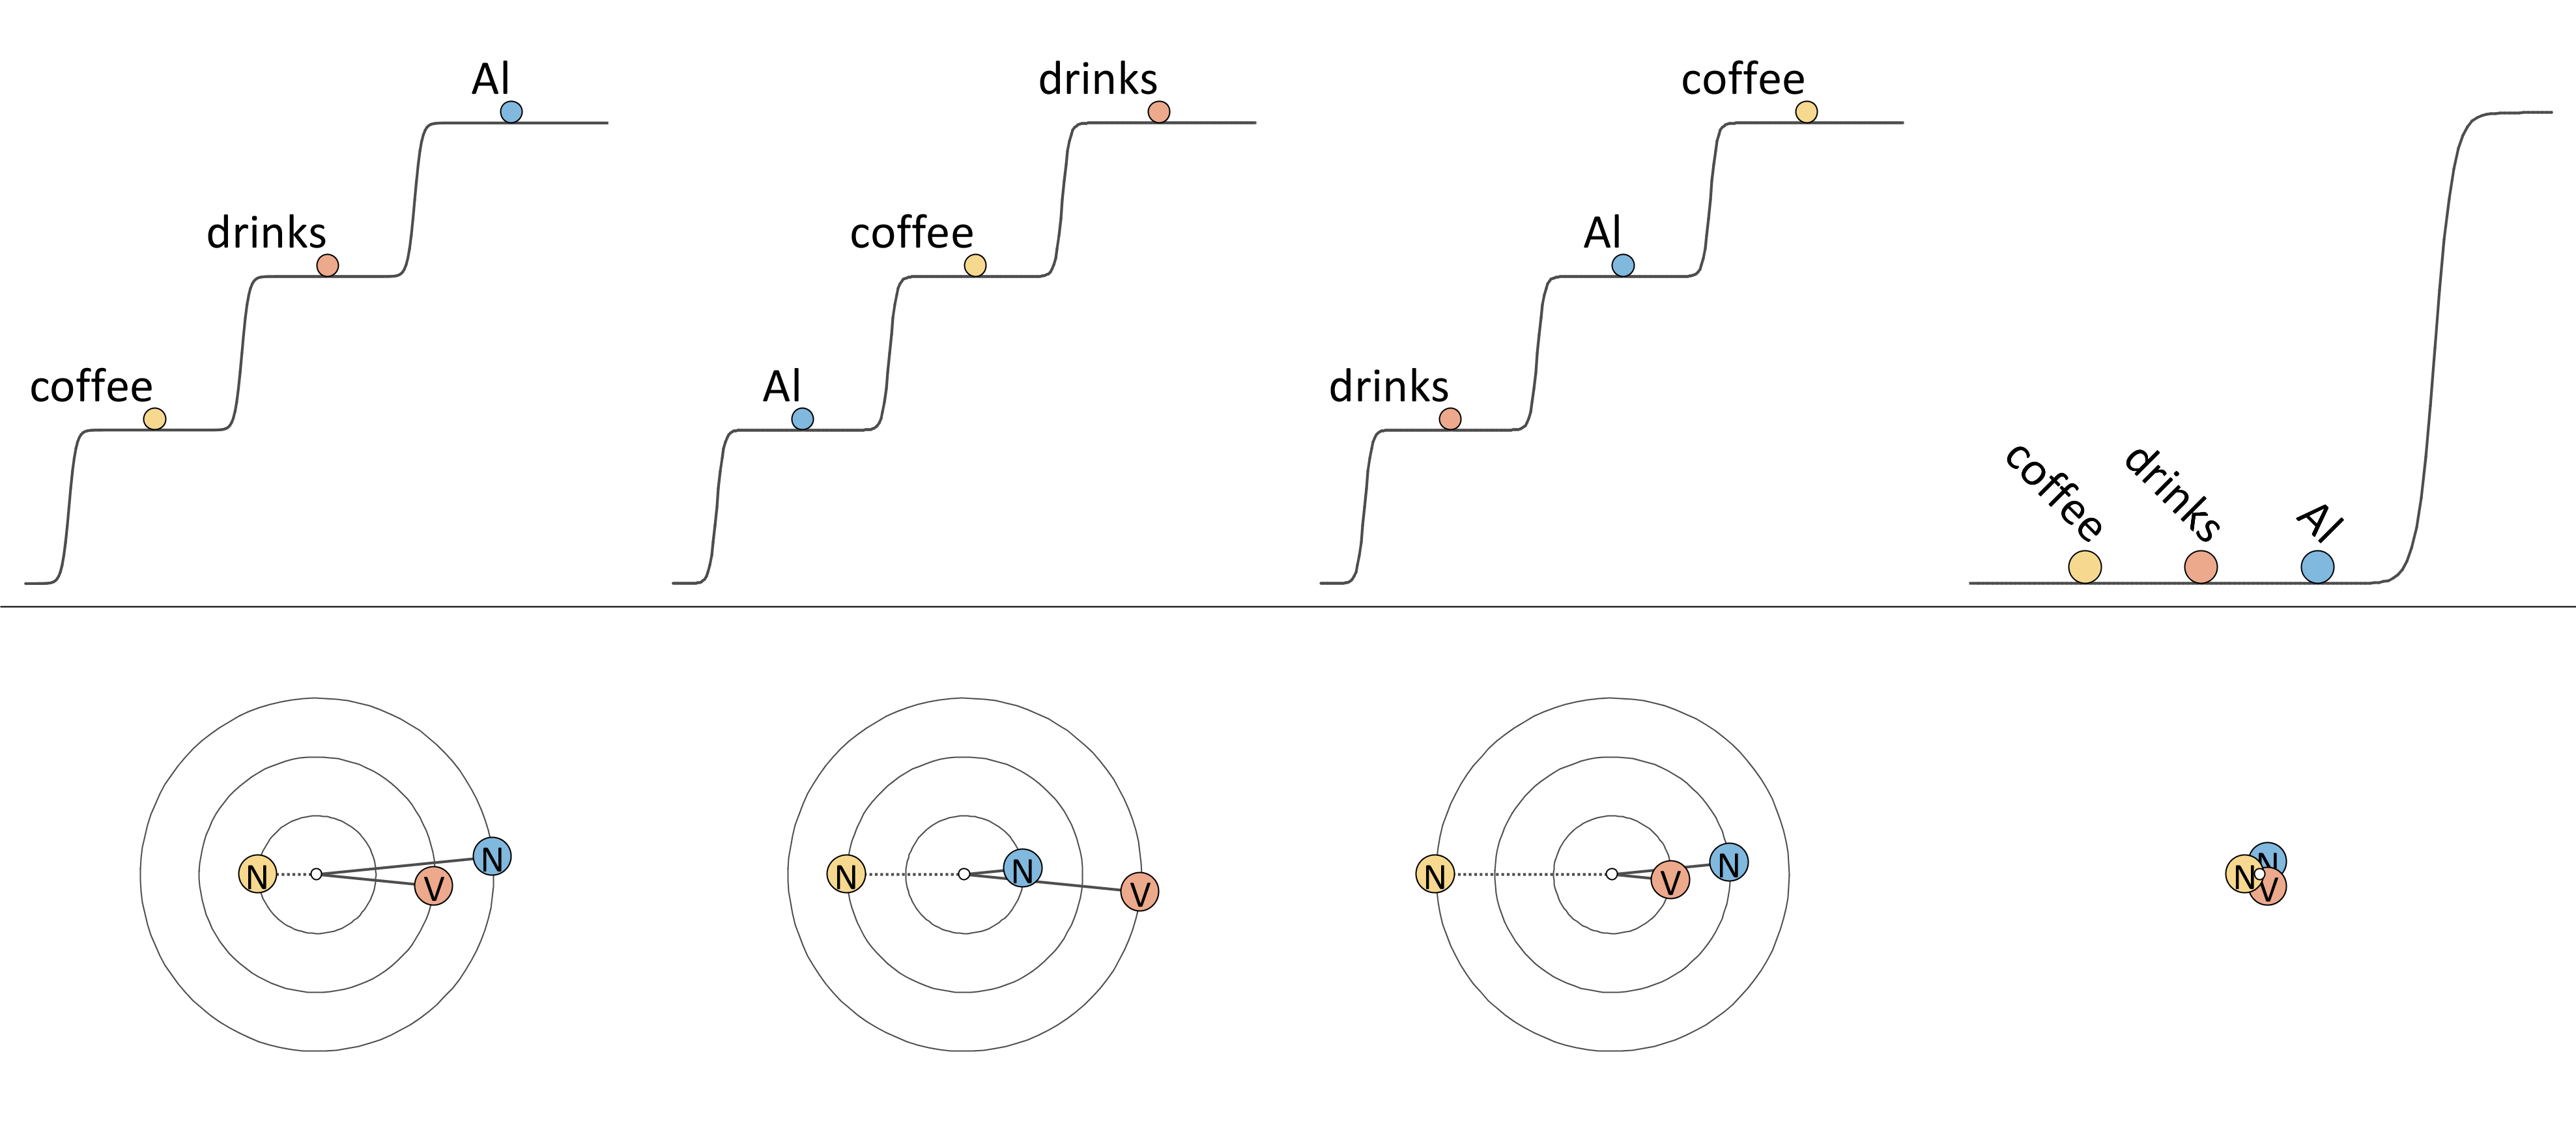
\includegraphics[width=\textwidth]{figures/Tilsen-img168.png}
\caption{Oscillator/energy levels representations are analytical constructs.}
\label{fig:8:2}
\end{figure}
 

  Both of these analytical representations—excitation potentials and orbits—evoke temporal schemas: the e-potentials remind us that e-organization forces maintain stable states and induce abrupt changes, resulting in discontinuous trajectories in e space. The orbits remind us of periodic trajectories in θ space and stable ϕ relations.

  For some readers, the forces we have constructed may seem too mystical—after all, these forces are not gravity, electromagnetism, etc. But nothing is particularly magical about integrating the effects of many synaptic interactions within and between neural populations, from which the forces are derived. The conventional entities—syntactic objects—are in many ways much more otherworldly than the forces constructed in the o/el framework. But regardless of whatever personal preferences one may have for specific metaphors, the physical program requires us to be conscious of those metaphors when we construct theories.

\section{Barriers to physical linguistics}

Freedom from object metaphors and generative thinking lets us explore new metaphors and alternative analytical representations. This may be useful, and if nothing else it is fun. But advocating for new metaphors usually brings new burdens. In the case of the o/el framework, the burden is responsibility to motivate the construction of a state space. We have not yet attempted to rigorously motivate our state space construction, and apart from some additional comments below, the hard work has been deferred. Instead, we have explored the state space as children explore a playground. In the process, we have tried to discover the workings of the playground apparatus. Will the o/el playground be useful for future investigators? Does the physical program gel with how practitioners of conventional approaches view language? Unfortunately, current theoretical approaches seem to be incompatible with the physical linguistics program, and this is unlikely to change in the near future. The most important barriers are social, and we catalogue them below.

\subsection{Structuralist performance}

One barrier is the performance of structuralist conceptualizing in linguistics, cognitive science, and psychology. This behavior is natural: we use metaphors and image schemas to develop constructs for thinking about the world, and those constructs are perpetuated through normal modes of scientific transmission, such as discussion, teaching, mentorship, and publication. By historical contingency, objects and container/connection schemas have become the dominant constructs. Thus linguistic units \textit{seem to be like} objects because we perpetually reconstruct object metaphor concepts, by using the metaphor in our discourse. This particular barrier would seem to be easy to overcome: we simply need to perform alternative modes of thinking, for example thinking in terms of oscillators and energy levels; states, trajectories, and forces; stability and interference, etc. Yet our habits can be difficult to change, and so it is unclear whether structuralist performance can be easily avoided. 

\subsection{Pretense of objectivity}

Another barrier, perhaps more fundamental, is the common attitude and mode of discourse in which linguistics and more generally, science, is understood to involve non-subjective observation of reality, and these so-called observations provide a basis for “falsifying” theories. This way of thinking is so ingrained in our folk theory of scientific practice that conscious, explicit rejection of it is not enough: deliberate careful appraisal of discourse is required to transcend it. The key is to recognize that “the world” and “reality” are always constructs, and more specifically that any “data”, “observations”, and “measurements” are always pre-determined by our conceptual models. This must be so on all levels of analysis. No matter how discomforting and antithetical to folk wisdom it may be, it must be embraced. The constructedness and contingency of our theories is not a problem, but rather, a solution. No complex thought would be possible if we were not able to blend schemas, transiently couple distinct networks of concepts into new, more interesting networks. The goal of any new conceptual model, such as the o/el framework, is to push our understanding into unexplored territory, by constructing new conceptual networks to use as analytical tools. In that spirit, it is frustrating to encounter discourse which drips with presuppositions of objectivity and certainty. For example, consider following regarding the question of what properties that are specific to human language:

\begin{quote} 
The questions arise in principle for any organic system, and have been raised since the early days of modern biology. The only general questions concerning them have to do with feasibility, not legitimacy. \citep[133]{Chomsky2008}
\end{quote}

Legitimacy by what authority? A more subtle example, where what is \textit{recognized} is assumed to be true by entailment:

\begin{quote} 
As has long been recognized, the most elementary property of language – and an unusual one in the biological world – is that it is a system of discrete infinity consisting of hierarchically organized objects \citep[134]{Chomsky2008}.
\end{quote}

\begin{quote} 
It has been recognized for thousands of years that language is, fundamentally, a system of sound-meaning connections; the potential infiniteness of this system has been explicitly recognized by Galileo, Descartes, and the 17th-century "philosophical grammarians" and their successors, notably von Humboldt \citep{HauserEtAl2002}.
\end{quote}

To suggest that every “constructive” approach presupposes your system of metaphors is a remarkable form of hubris:

\begin{quote} 
…A stronger thesis is that the biolinguistic approach has a kind of privileged status, in that every constructive approach to human language and its use presupposes it, or something similar, at least tacitly. \citep{Chomsky2001a}
\end{quote}

  In the physical program, we aim to construct useful, and perhaps fun, conceptual models. If those models are indeed useful and fun, discourse which exhibits a pretense to an objectively correct understanding of reality should be unnecessary.

\subsection{Anthropocentrism}

Another obstacle to the physical linguistics program is the conviction that humankind and human thought is special. Glorification of human as opposed to animal behavior is pervasive but always misguided:

\begin{quote}
Why did humans, but no other animal, take the power of recursion to create an open-ended and limitless system of communication? \citep{HauserEtAl2002}.
\end{quote}

\begin{quote} 
Extraordinary acts of creation by children do not require the extraordinary circumstances of deafness or plantation Babels. The same kind of linguistic genius is involved every time a child learns his or her mother tongue \citep{Pinker2003}.
\end{quote}

  I have spoken with plenty of young children, and “genius” is not the word I would use the describe their communication abilities. The stimuli that children experience in development are only impoverished when one assumes a set conception of language: it is a no-brainer that the vast majority of the objects in an “infinite set” will not be encountered by a child. It is also troubling that reverence for human behavior is central in much of the conventional rhetoric. Consider the perspective of the Martian imagined in \citet{HauserEtAl2002}:


\begin{quote}
If our martian naturalist were meticulous, it might note that the faculty mediating human communication appears remarkably different from that of other living creatures; it might further note that the human faculty of language appears to be organized like the genetic code-hierarchical, generative, recursive, and virtually limitless with respect to its scope of expression. \citep{HauserEtAl2002}.
\end{quote}

  What is remarkable here is that the authors assume the Martian would come to these conclusions, i.e. that language is “hierarchical”, “generative”, “recursive”, and “infinite”? Clearly the authors have anthropomorphized the Martian, imposing their own conceptual framework on an entity that could think in vastly different ways from us. The same bias is applied to comparisons of human and non-human animal behavior:

\begin{quote}
Most current commentators agree that, although bees dance, birds sing, and chimpanzees grunt, these systems of communication differ qualitatively from human language. In particular, animal communication systems lack the rich expressive and open-ended power of human language (based on humans' capacity for recursion). The evolutionary puzzle, therefore, lies in working out how we got from there to here, given this apparent discontinuity. \citep{HauserEtAl2002}.

Although many aspects of FLB [\textit{broad faculty of language}] are shared with other vertebrates, the core recursive aspect of FLN [\textit{narrow faculty of language}] currently appears to lack any analog in animal communication and possibly other domains as well. \citep{HauserEtAl2002}.
\end{quote}

  There is a value judgment implied by phrases such as “lack the rich expressive and open-ended power.” From a more neutral perspective, we as researchers analytically construct understandings of the systems which govern non-human animal behavior, in the same way that we do so for human behavior. We can then compare those systems. Nothing about this analytical comparison requires us to think of humans as special and animals as lacking.

  Closely related to the anthropocentric stance are untenable interpretations of consciousness and intention. The notions that human consciousness is a special phenomenon, that we have “true” agency, and that we can “intend” to produce utterances—these run contrary to the physical perspective. There is no such thing as intention in the physical program. System states evolve under the action of forces, and no imp is necessary to make it happen. Anything that does not fit into that conceptual framework is dualist magic. That we \textit{believe} that we \textit{intend} to act must be a consequence of how the surroundings interact with our conceptual and motor systems. We do not experience all of the individual microscale forces which determine the evolution of the system; instead, we experience the aggregate effect of those forces. Sometimes those forces result in actions, such as speaking or writing. We interpret the experience of this as an “intention” to communicate, but the notion that we played the role of an agent in this process is an illusion.

\subsection{Hidden dualism}

Superficially, mind-body dualism has been loudly rejected in the biolinguistic program, and it seems to be frowned upon more generally in the communities of linguistics and cognitive science. In spite of this, dualism is alive but well-hidden. When there is subtle dualism, it is important as a coping mechanism to suppress any hints of it. The so-called narrow faculty of language (FLN) is, in all of the ways that matter, “the mind”, constructed in opposition to “the body”. Consider the following, regarding the relation of FLN to the sensory motor (SM) and conceptual intentional (CI) systems:

\begin{quote}
Faculty of language-narrow sense (FLN). FLN is the abstract linguistic computational system alone, independent of the other systems with which it interacts and interfaces. \citep{HauserEtAl2002}.
\end{quote}

\begin{quote}
We propose in this hypothesis that FLN comprises only the core computational mechanisms of recursion as they appear in narrow  syntax and the mappings to the interfaces (i.e. the interfaces with mechanisms of speech perception, speech production, conceptual  knowledge, and intentions) \citep{HauserEtAl2002}.
\end{quote}

  Depending on how we interpret certain words in the above statement (i.e. \textit{abstract}, \textit{independent}, \textit{system}, \textit{interacts}, and \textit{interfaces}), the concept of the FLN is either nonsensical or just a rhetorical strategy for concealing dualism. First, what does “abstract” mean here? It cannot mean non-physical. But what would a \textit{non-abstract} “linguistic computational system” be? What makes the system \textit{abstract}, rather than \textit{concrete}? Most dictionaries would suggest that by calling something “abstract” we say that it exists in thought or as an idea but does not have a physical or concrete existence. Is that the sort of abstractness that the authors imply? If so, we have a dualistic conception. 

  Much more problematically, what do the authors mean by stating that the system is \textit{independent} of other systems, but nonetheless \textit{interacts} and \textit{interfaces} with them? It seems reasonable to substitute \textit{independent} with “not influenced by”. Does this gel with an interpretation of \textit{interaction} and \textit{interface} in which interactions and interfaces between systems are bidirectional? Obviously not, because \textit{independence} contradicts \textit{interaction} and \textit{interface}: FLN cannot simultaneously be influenced by other systems and not be influenced by those systems. The other possibility is that interactions and interfaces are unidirectional influences: FLN can influence SM/CI but not vice versa. If so, we are again in dualist territory. 

  The point is that one cannot have it both ways. One cannot pretend that a system is isolated from other systems, and at the same time insist that one has no such pretension. Closeting the surroundings into acronyms like SM and CI is a deceptive maneuver, or more generously, results from a lack of self-awareness. In the physical program, we are perpetually aware that our construction of the systems and surroundings is \textit{always} an analytical construction, and this helps us remain vigilant against hidden dualism.

\section{The art of analytical construction}

The o/el framework is constructed from metaphors and image schemas, just as the conventional approach is. All theories can be deconstructed from this perspective. If we pursue a deconstruction of the o/el framework, we find a hierarchy of metaphors and schemas, such as below. 

  
\begin{figure}
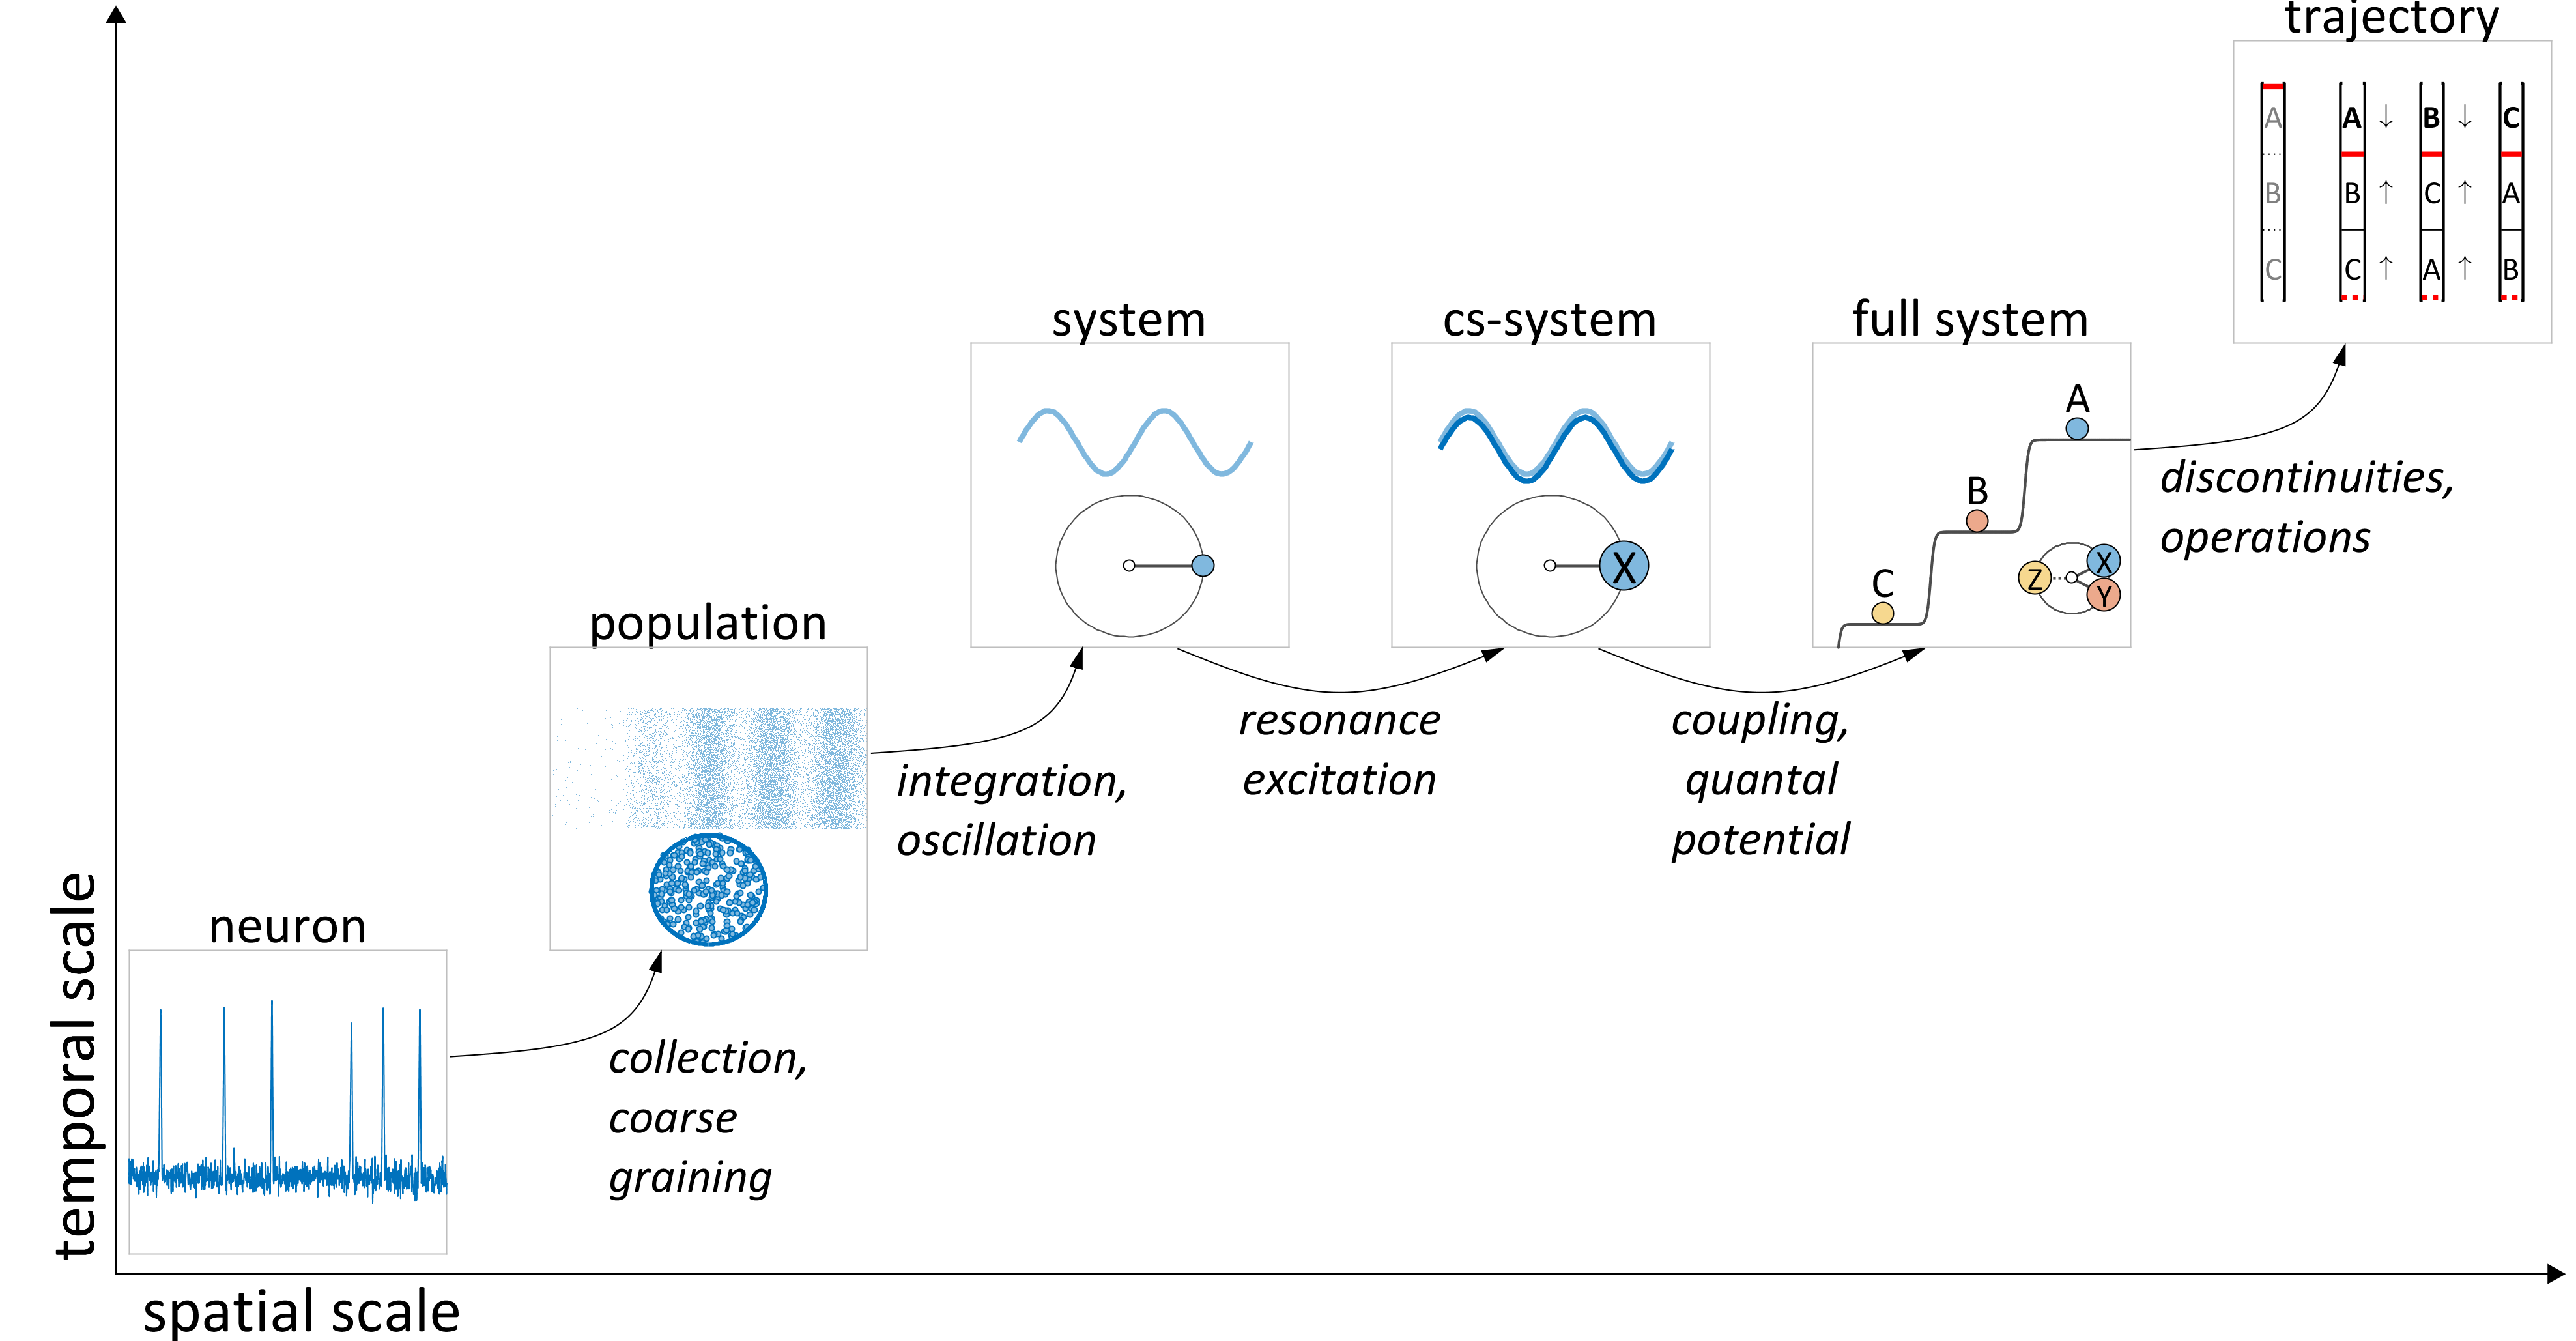
\includegraphics[width=\textwidth]{figures/Tilsen-img169.png}
\caption{Hierarchy of metaphors and image schemas used to construct system trajectories.}
\label{fig:8:3}
\end{figure}
 

  On the largest scale, we locate the analytical construction of a ϕ,e state space trajectory for the full system. The full system trajectory is constructed by discretizing time and operating on full system states. The full system state is constructed by imposing concepts of phase coupling on cs-system interactions and discretizing relative excitation of cs-systems with a quantal excitation potential. The cs-systems are constructed by imposing concepts of resonance and excitation on a smaller spatial scale corresponding to c-systems and s-systems. The c- and s-systems are in turn constructed by integrating over patterns on a smaller spatial and temporal scale associated with neurons in populations, and by imposing an order parameter with oscillatory and non-oscillatory components. Populations are constructed by integrating and coarse graining in space and time on the neuronal scale. Even the concept of a synapse is an analytical construction—on what basis should one consider the axon terminals of one neuron and dendritic neurotransmitter receptors as a single, functional system, rather than composites of a multitude of molecular-scale subsystems? 

  On all scales, theoretical constructs are relatively macro-scale descriptions of relatively micro-scale patterns, made possible by more or less conscious decisions to impose metaphors and schemas. When we choose to construct an understanding, rather than pretend to discover it, we make these decisions more consciously. All analyses become \textit{impositions}, in that we impose the analysis on phenomena which are otherwise unanalyzed. We do have an obligation to motivate analytical impositions, although in practice this is difficult and holding ourselves to overly high standards is counterproductive. The are two main reasons for the difficulty. 

  First, any rationale one could provide must presuppose, or better, establish, a shared system of values or objectives. Maybe our theories should be useful (but for what?), or predictive (but of what?). Maybe they should be productive (in what way?). Perhaps they should be creative, or aesthetic (to whom?). Perhaps they should be fun (for whom?). Or liberating (from what?). A shared basis for valuing analyses is needed. Second, we lack a detailed understanding of the systems-level organization of the nervous system. The o/el framework tries to extrapolate from population coding, collective oscillation of networks, and varieties of synaptic interaction, but these extrapolations are admittedly tenuous and speculative. Hopefully future theories can provide a more detailed derivation of macro-scale analyses from the high-dimensional state of the nervous system. Some useful tools for such an endeavor are described in the following section.

\subsection{Tools of state space construction}

To derive the o/el model we start with a profoundly detailed, high-dimensional picture, a space where the dimensions correspond to the electrical currents/voltages, ion channel states, and chemical flows/gradients at a very fine spatial and temporal resolution throughout the entire nervous system, for all organisms, along with the acoustic pressures, spectra, etc. of the local environments of all those organisms. (Of course, we have already imposed some constructs invoking macroscopic notions of pressure, gradients, voltages, spectra, etc., and these provide lower bounds on spatial/temporal resolution.) 

  After we imagine the profoundly high-dimensional space, we proceed to reduce its dimensionality to better suit our interests in linguistic phenomena. Two of the most fundamental tools for dimensionality reduction are projection and integration. Some examples of linear projections (specifically, orthogonal ones), are shown below. In {\figref{fig:8:4}}(A), two states are shown in a three-dimensional space. By projecting these states onto a two-dimensional plane, we ignore variation in the third dimension. The similarity of projected states depends on which dimensions are retained/discarded in the projection. The same projection operations can be used for trajectories, as in {\figref{fig:8:4}}(B): projecting over dimension 3 lets us focus on the periodic variation in dimensions 1 and 2.

  
\begin{figure}
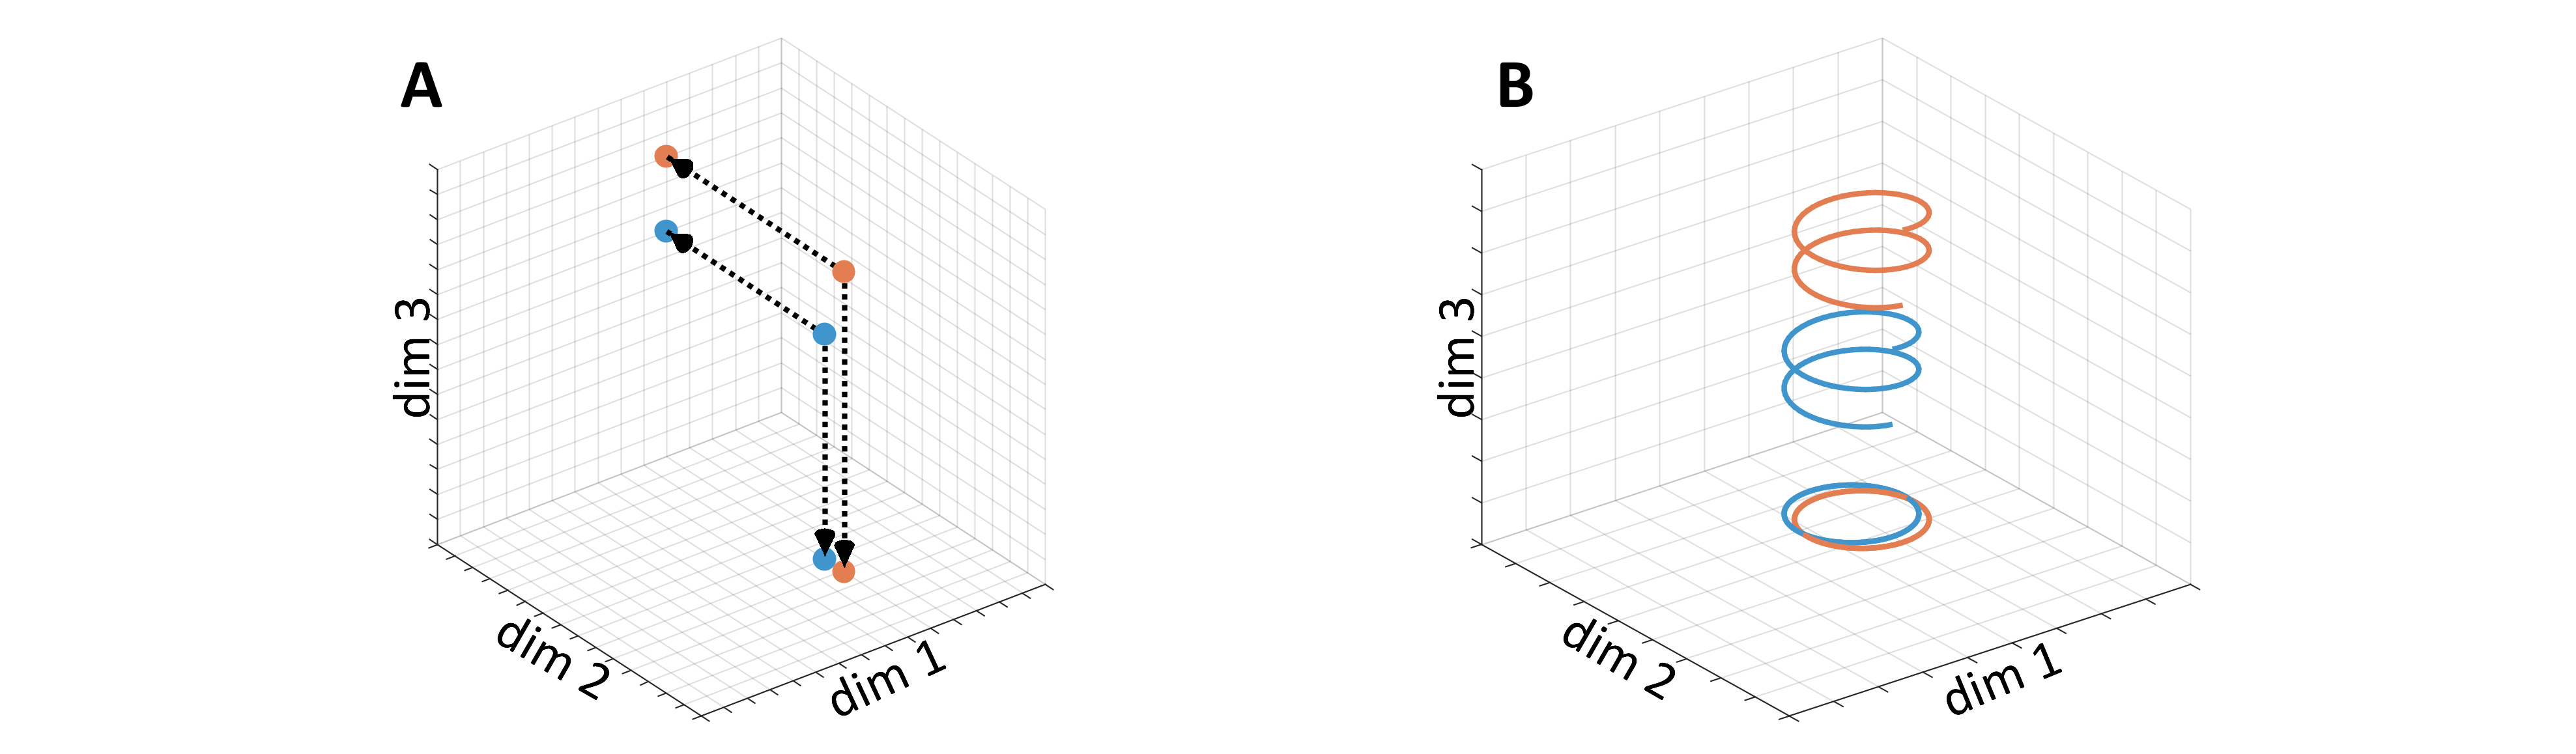
\includegraphics[width=\textwidth]{figures/Tilsen-img170.png}
\caption{Projections of states/trajectories from higher-dimensional spaces to lower-dimensional spaces.}
\label{fig:8:4}
\end{figure}
 

  Projection lets us choose to ignore some dimensions of state space (i.e. degrees of freedom). This help us focus on the information we suspect to be relevant. In many circumstances, a dimension is irrelevant because the information it is associated with interacts weakly with information we have chosen to be interested in. The forces and systems we construct do not depend on many of the high-dimensional state space dimensions. 

  The other main tool we have is integration/coarse-graining/averaging. In a non-technical sense these are different names for effectively the same procedure. Whereas orthogonal linear projections remove dimensions from state space, integration combines dimensions to construct new ones. Integration is a powerful tool because it lets us choose the spatial and temporal scales on which we construct analyses. Through strategic choices of scale and state-space re-structuring we construct new dimensions which are more useful for analyses. Examples of temporal and spatial integration are shown in {\figref{fig:8:5}}(A) and (B). Observe that on the longest timescale in the temporal integration we can more clearly see a step-like change in a quantity, whereas the intermediate scales better show periodicity.

  
\begin{figure}
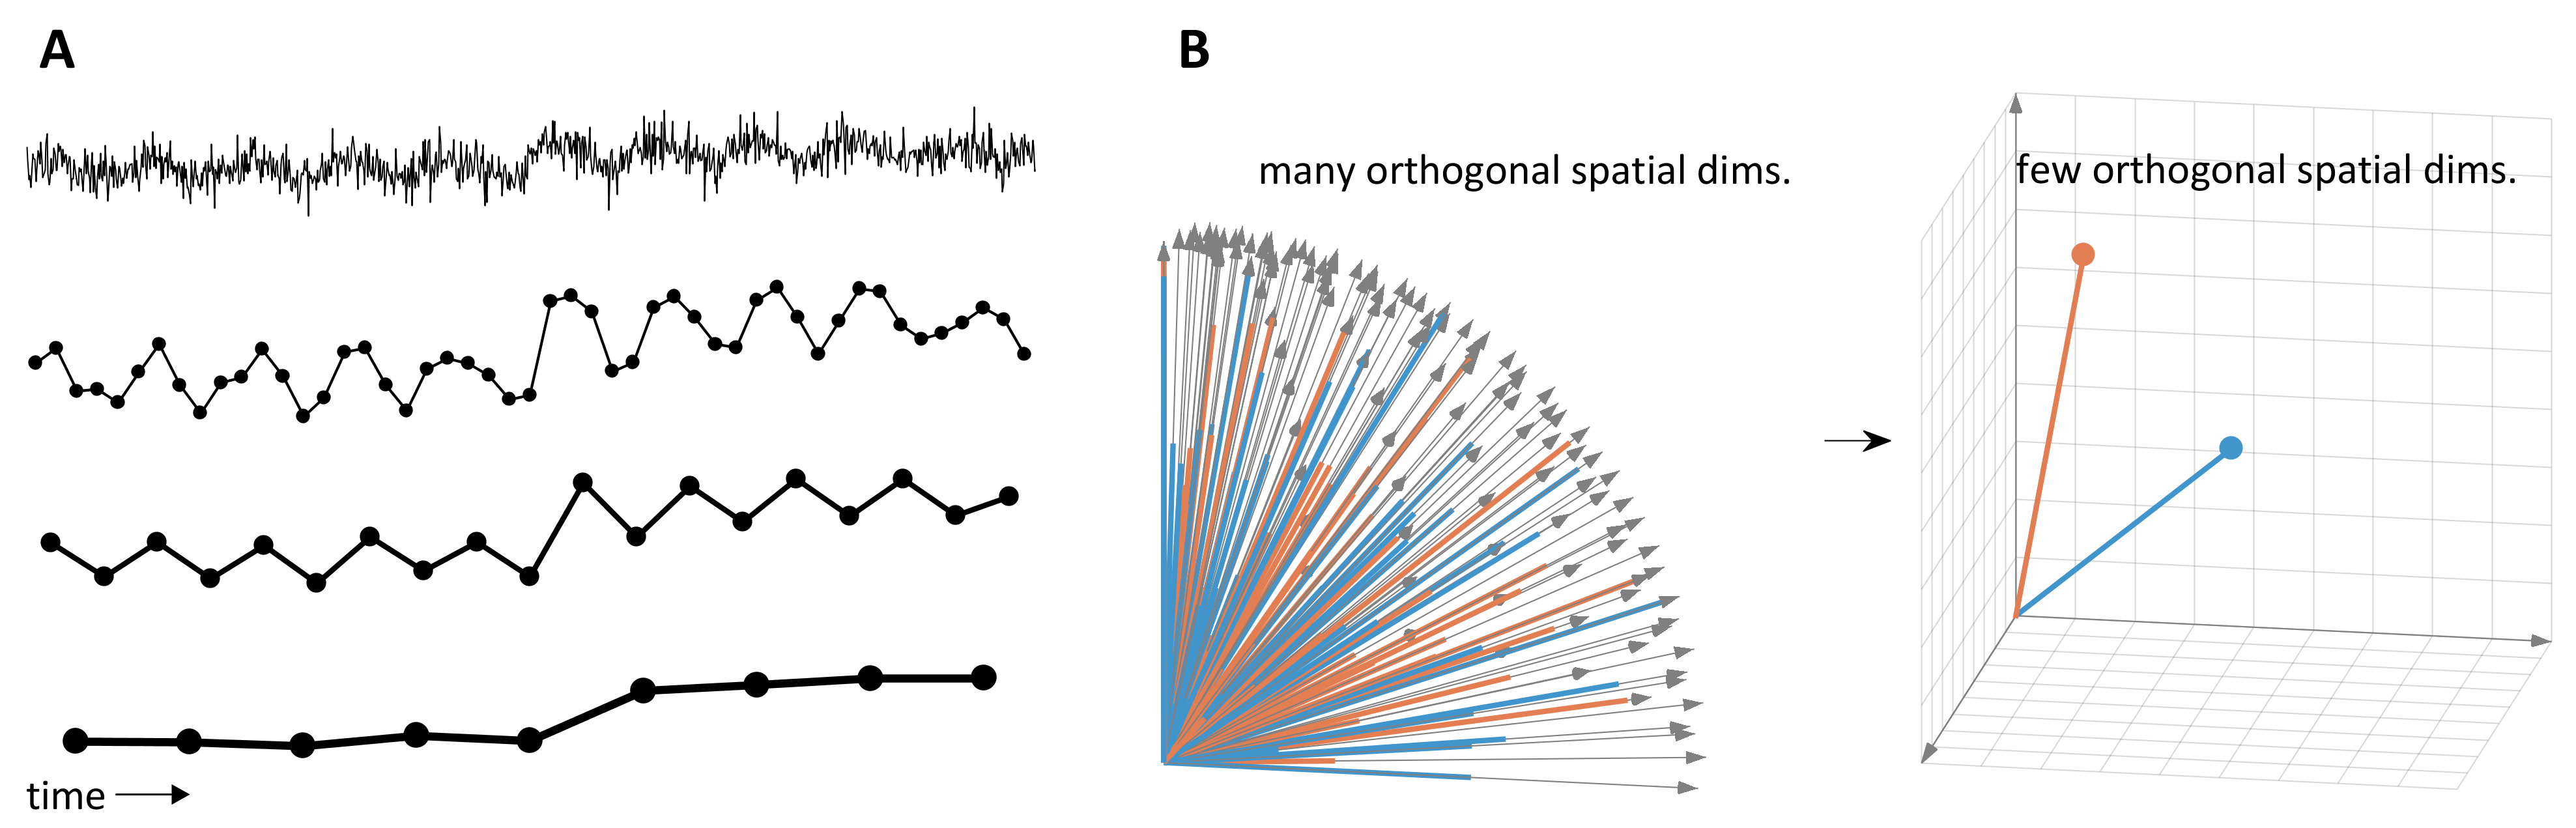
\includegraphics[width=\textwidth]{figures/Tilsen-img171.png}
\caption{Coarse-graining in time and space.}
\label{fig:8:5}
\end{figure}
 

  There is an interesting difference in how we tend to integrate over space vs. over time. In a temporal integration, each time step is a separate dimension, and we typically preserve an ordering of those dimensions. In contrast, when we perform spatial integration, we have more freedom to pick and choose dimensions and thereby scramble spatial information.

To see the utility of these tools, lets consider an example, the concept of neuron as \textit{node} in a network. In the connectionist tradition, it is common to conceptualize a neuron as a system which produces output in response to some input, and the brain is understood to be comprised of many such systems, potentially interacting with each other. How can we derive the construct of a neuron, and of interaction between neurons, from the higher dimensional state space of the nervous system? Imagine that we have no idea “what” a neuron \textit{is}, but we can measure voltages and chemical gradients in the nervous system with high spatial and temporal resolution. By statistical examination of these quantities when integrated over a range of spatial and temporal scales, we could “discover” the neuron from the dependence of correlations on integration scale: we could find that, in a probabilistic sense, there are particular spatial and temporal scales which are optimal for distinguishing certain patterns of measurements. The optimal scales are those which integrate out irrelevant fluctuations, but are no larger than characteristic scales of variation associated with the pattern.

  The concept of “a language” is another example. What \textit{is} a language, e.g. English? You cannot observe it or measure it; it does not occupy space or contain objects. Clearly it is an analytical construct, but to what extent is it a useful construct, and how could we derive it? Imagine that we have no idea “what” a language is, but we can measure acoustic signals produced by people at all locations in space and time. As with the neuron, by examining these signals statistically over a wide range of spatial and temporal scales, we could “discover” languages: we would find that, there are particular spatial and temporal scales of analysis which optimize certain correlations or contrasts between patterns. The contrast optimization is necessarily relative to which patterns we, as analysts, find relevant. This is why there is no pre-theoretical notion of a language.

  In general, our analytical constructs—neurons, neural populations, words, people, social networks, dialects, languages, language families, etc. can be understood as consequences of scale non-invariance. Quantities of interest, as we integrate them over larger and larger scales, tend \textit{not} to be renormalizable with simple scaling laws. Most likely this is because of strong interactions between systems across a range of scales; in other words, because of complexity. The good news is that scale non-invariance provides a rationale for \textit{choosing} scales of analysis: our analytical impositions can be tailored to optimize correlation or contrast in some interesting quantities.

\subsection{Thermodynamics of speech}

While projections and integrations are useful tools for analytical construction, there is also much value in exploring physical analogies. One idea I find compelling is that, from a physical perspective, speech and biological life have a lot in common. Physicist Erwin Schrödinger gave a famous lecture series on the physical nature of life, which was later adapted to a book \textit{What is Life?}. Schrödinger wrote:

\begin{quote}
Life seems to be orderly and lawful behaviour of matter, not based exclusively on its tendency to go over from order to disorder, but based partly on existing order that is kept up. To the physicist—but only to him—I could hope to make my view clearer by saying: The living organism seems to be a macroscopic system which in part of its behaviour approaches to that purely mechanical (as contrasted with thermodynamical) conduct to which all systems tend, as the temperature approaches absolute zero and the molecular disorder is removed. \citep{Schrödinger1944}
\end{quote}

  To paraphrase loosely, what makes life unlike many physical systems is its counteraction of the second law of thermodynamics: instead of increasing entropy, i.e. distributing energy/matter more evenly in space and time or causing the probability distributions of system microstates to become more uniform, living systems maintain and increase order locally by transformations of energy collected from their environment. To say that life counteracts the second law is not saying that the second law is violated, of course—entropy always increases for the universe as a whole. But living systems are particularly good at maintaining spatially and temporally local concentrations of energy and restricting the number of microstates which are accessible to them. In other words, life maintains and perpetuates itself by creating order. Physicist Ilya Prigogine showed how order can emerge in systems driven far from equilibrium (\citealt{KondepudiPrigogine1998,NicolisPrigogine1977,PrigogineStengers1984}), and recent work by Jeremy England and colleagues has shown how driven, nonequilibrium systems may adapt to absorb work from their environment:

\begin{quote}
We point out that the likelihood of observing a given structure to emerge in nonequilibrium evolution is strongly influenced by the amount of absorption and dissipation of work during its history of formation. We examine the mechanism of this general relationship in simple analytical examples. Subsequently, taking inspiration from the way evolutionary adaptation is understood in a biological context, we argue that many structures formed far from equilibrium may appear to have been specially selected for physical properties connected to their ability to absorb work from the particular driving environment, and we discuss the relevance of this hypothesis to studying the physics of self-organization \citep{PerunovEtAl2016}.
\end{quote}

  If physicists are on to something about the evolution of life, perhaps the same ideas apply to language. On the scale of neural populations, the conceptual and syntactic systems in the o/el conception—when excited—are far-from-equilibrium and highly ordered: collective oscillation of a population is a dramatic local reduction in entropy. This order creation is possible because individual neurons are adapted to absorb work, in the form of electrochemical gradients maintained across cell membranes, and are adapted to collectively oscillate via their synaptic interactions and local circuitry. Linguistic behavior on the utterance scale, rather than maximizing entropy, necessarily reduces entropy in a local sense. The timecourse of production, as we have conceptualized it, begins from a relatively disordered initial condition, evolves toward a more ordered steady state, and subsequently transitions from steady state to steady state in a highly predictable way. 

  The distributions of these ordered states and the distributions of the transitions between them are highly non-uniform. This raises the question of whether the forces which influence those distributions on larger scales—i.e. over the lifetime, and diachronically—are also order-creating. Clearly our genetic inheritance—a product of evolutionary scale forces—is a physical system which learns to induce ordered states. The crucial question is whether we can understand these patterns—e/ϕ configurations—as \textit{adapted} to extract work from the surroundings.

  From this perspective, let's consider the historical-scale phenomenon of grammaticalization, which can be viewed as the emergence of a grammatical s-system from a lexical one. A common diachronic trajectory is one in which adverbs and adpositions become verbal tense/aspect and agreement markers (\citealt{HeineKuteva2002,TraugottHeine1991}). These diachronic trajectories can be interpreted as evolution of the corresponding \{A\textsc{dv}\} and \{P\} systems so as to more efficiently absorb excitation from a \{V\} system. First, consider that the coupling of an excited \{V\} system to \{A\textsc{dv}\} and \{P\} entails that \{A\textsc{dv}\} and \{P\} experience an oscillatory driving force from \{V\}. In other words, \{V\} is part of the “environment” of the \{P\} and \{A\textsc{dv}\} systems and \{V\} does work on them. Let's furthermore assume that s-systems organized on the same e-level are more strongly coupled than s-systems which are organized on different levels. In that case, the evolution of \{A\textsc{dv}\} and \{P\} to be co-selected with \{V\} correlates with an increase in the extent to which \{A\textsc{dv}\} and \{P\} are excited by \{V\}. Crucially, because the g-domains and gm-organization of systems can be conditioned on how they are e-organized, we would expect that \{A\textsc{dv}\} and \{P\} may come to excite different g-domains in the co-selected vs. competitively selected organizations. This difference in organization may facilitate the differentiation of \{\textsc{tense}\}/\{\textsc{aspect}\} and \{\textsc{agreement}\} grammatical s-systems from lexical \{A\textsc{dv}\} and \{P\} systems, and in turn facilitates the differentiation of associated c-systems. 

One question that the above analysis raises is what prevents such grammaticalization processes from happening more pervasively. Perhaps configurations which extract too much work or create too much order may be maladaptive for reasons that are not yet apparent. Moreover, organizing too many systems in the same e-level results in destabilizing interference. In any case, a thermodynamic approach to understanding diachronic changes in system configurations holds a great deal of explanatory potential.

\subsection{Perspective shifts}

A useful technique for cultivating intuitions in the physical program is to conduct thought experiments in which one attempts to imagine how analytical constructs, when deliberately personified, would experience phenomena. For example, how do syntactic and conceptual systems experience time? 

  To pursue this question we consider what the experiences of such systems could be like, given how we have constructed them. (We avoid getting hung up on defining “experience” here). Syntactic and conceptual systems are relatively macroscopic entities, so we imagine that they do not experience microscale phenomena such as individual synaptic flows or neuronal depolarizations. We also presume that these systems \textit{do} experience variation in their internal e and θ states, and have an experience of forces from other systems and the surroundings. If we assume that systems are not aware of their own parts and do not differentiate the sources of their interactions, we infer that systems experience only an aggregate force. 

  Systems \textit{do} have memories, in a sense: some system parameters vary slowly relative to the system state; these slowly varying parameters influence and are influenced by faster varying parameters of the system state. We can think of memory as the consequence of interactions between relatively slow timescale processes and relatively fast timescale processes. One such memory parameter is the intrinsic frequency \textit{f} of the oscillatory component of the system order parameter. The intrinsic frequency influences the instantaneous frequency of a system, and stable coupling of systems requires mutual approximation of the instantaneous frequencies, i.e. frequency-locking. Intrinsic frequency may be related to microscale state variables such as population size and intrapopulation connectivity. Presumably these microscale variables have both slow (memory-like) and fast dynamics. Fast variation in production (e-organization) may outweigh slow variation generally. On supra-utterance scales, \textit{f} variation may also interact with system capacities, i.e. maximal population sizes. 

  Another memory-like parameter is intrinsic \textit{susceptibility χ} to forces from other systems and the surroundings. The susceptibility can be viewed as a component of the coupling strengths $\Phi$ and $\epsilon$ introduced previously. We imagine that slow micro-scale variation in the relative proportions and/or strengths of inhibitory and excitatory projections between populations, and the number of such projections relative to system size, manifests as slow variation in how a population responds to forces.

  Having posited that systems experience internal e and θ states, experience forces on those state variables, and have memories in the form of intrinsic frequencies \textit{f} and intrinsic susceptibilities \textit{χ}, we can now address the original question: how do systems experience time? In the o/el framework, this experience must be quite bizarre. There are long periods of time in which systems are “asleep,” i.e. inactive, having no awareness of their internal states. The systems do not really exist during these periods, in some sense, because there is no collective oscillation. In the pre-stable phase of production, systems awaken to tumultuous changes in their internal states, driven by an external force which is chaotic and unpredictable. Time is problematic to define in this condition because there are no quantities that change predictably. Many systems may either lose consciousness or remain in this state for a while. 

  Some systems will undergo a transition to a vastly more predictable experience of time in which e is constant and θ changes with nearly constant angular velocity. For a system in this boring, stationary regime, time is experienced not in a linear fashion, but rather as periodic, because the only internal state that varies is θ. As a consequence of time translation symmetry, the system will have no awareness of a global past or future; instead, the system will only be aware of local progression of θ states. 

  We can also consider how the system experiences net forces in this state. Consider that ϕ forces influence phase velocity dθ/dt = $\dot{\theta}$, and because the system is in a stable steady state, both e and $\dot{\theta}$ are at stable equilibria. This entails that the net external e and ϕ forces experienced by the system average to zero. Yet there are fluctuations in all systems and in the surroundings, and so the net force on any given system will fluctuate and perturb the system from its equilibrium. The system will experience a force which counteracts the perturbations of $\dot{\theta}$ and e. The stronger the fluctuations, the greater the perturbations, the more noticeable the stabilizing force. Because interference manifests as a perturbation of $\dot{\theta}$ and e, a system experiences interference as a perturbation from and subsequent return to an equilibrium—in other words, the system experiences confinement to a particular region of its state space.

  The typically uneventful e-epoch does not persist indefinitely. In canonical trajectories, the system experiences intermittent abrupt transitions to new steady states. The transition is too abrupt to experience as temporally non-uniform. So as far as the system is concerned, its e state changes instantaneously. This also renders any global experience of time problematic to define. In normal circumstances the timing of the transitions cannot be anticipated. Hence the system cannot predict when these catastrophic state changes occur. In contrast to the e state, the system experiences no evidence of discontinuity in θ. Hence the experience of the system over a canonical utterance trajectory depends on which internal state variable we consider. The phase θ variable rotates uniformly, with small perturbations of $\dot{\theta}$. This is an invariant experience. The excitation e variable remains constant most of the time but intermittently jumps to new values. This is sort of like riding a roller coaster that is always corkscrewing.

\subsection{Open questions and speculations}

Most of the macroscale concepts we constructed in the preceding chapters were based on conjectures derived from a limited understanding of microscale systems. A variety of simplifying assumptions were imposed for the sake of developing a workable framework. Questioning these impositions is worthwhile, as is speculating on alternatives or extensions.

  For one, it is far from clear how collective oscillation should be modeled on the macroscale. Collective oscillation of neural networks has been extensively researched in the lab and in simulations; yet the laboratory research does not currently have the combination of spatial resolution and coverage necessary to differentiate in the brain the systems we have postulated in o/el framework, and the simulations require many assumptions which can be called into question. The simplest picture of a collective oscillation (putting aside population size for the moment), and the one we imposed in most analyses, is a harmonic oscillation.

  This idealized harmonic oscillation almost certainly misses important information. For example, we could consider a more detailed microscale model in which populations are comprised of subpopulations which correspond to polychronous groups (cf. \citealt{Izhikevich2006}). The polychronous groups are subsets of the population that exhibit a particular spatial-temporal pattern of firing. The presence of such subpatterns would suggest that we reinterpret the collective oscillation as an integration of many oscillations, and this requires a macroscale conception of an oscillation spectrum. (Indeed, we stipulated that each system has a spectrum of this sort in developing a concept of the spectral coherence of a system.) Exactly how to derive an order parameter whose oscillation component has this property is an open question.

  Furthermore, systems may have multiple modes of oscillation, creating interesting possibilities for within- and between-system interaction. Within a single population, interactions between the oscillatory modes could be important, and this seems consistent with empirical studies which show that high-frequency (gamma-band) oscillations are modulated by the amplitude of theta-band oscillation. Moreover, multi-mode oscillations bring a host of new possibilities for interference between systems, with consequences for stability. One crucial question we have not resolved is whether differentiation of a system is accomplished through phase modulation, frequency modulation, or some combination of both. It is possible that systems participating in a non-attended but nonetheless active ϕ configuration must lock to a frequency that differs from the frequency of attended systems.

  A number of other speculations could be worth exploring. One involves the relation between oscillation frequencies and excitation. For a quantum harmonic oscillator in a potential, energy is quantized and proportional to frequency, with the set of frequencies being determined by the size of the potential. One might think of excited s-systems as such: their frequency corresponds to a ground-state wavelength determined by population size, and excitation levels are proportional to integer multiples of the ground-state frequency. In contrast, c-system frequencies are less strongly quantized and adapt to s-system frequencies via the resonance mechanism. Along these lines, our microscale conception of c-systems as spatially distributed and s-systems as relatively spatially localized suggests a model of s-systems oscillations in a 2D medium such as a circular membrane, i.e. a drumhead. There are both axisymmetric modes of vibration (determined by the radius of the membrane) and nonaxisymmetric modes. If we take the microscale conception of s-systems seriously, the membrane model could be useful.    

  One of my favorite speculations is that the emergence of the collective oscillation in a neural population is analogous to a turbulent inverse cascade. When energy is injected non-homogeneously at small scales, shear forces (i.e. asymmetries in interneuronal coupling) create small-scale vortices (polychronous subpopulations) which combine into larger- and larger-scale vortices, until reaching a maximal scale determined by the system boundaries. The emergence of collective oscillation seems quite similar to this. Even more remarkably the large scale vortices/oscillations stabilize by interacting with one another in highly constrained ways. Without these multi-scale interactions, transient stability could not be achieved.

\section{Learning and innateness}

A major topic which has not been addressed thoroughly in this book is how conceptual-syntactic patterns are learned, and to what extent aspects of the o/el model are innate or acquired through experience. A more comprehensive framework should provide explicit mechanisms and conditions for learning. It is important to note that any attempt to understand learning is necessarily colored by a conceptualization of \textit{what}, specifically, is being learned. Attempts to model learning which presuppose a conventional vision of syntactic-conceptual organization can only be successful to the extent that the object-based conception is useful. Thus, it stands to reason that a more useful understanding of adult linguistic behavior will inform the study of language development. In other words, investigation of learning depends on a notion of \textit{what} is learned. By proposing a number of explicit ideas regarding our conceptualization of language, the o/el framework provides a new basis for the investigation of learning. Below we briefly consider some examples of how this may play out, but first we touch upon a more philosophical issue revolving around the origins of human behavior.

A common debate in modern discourse pits learning vs. innateness as the source of linguistic behavior. This debate is flawed in the current perspective because all behaviors must result both from the physical substrate which generates them—e.g. neural populations in the brain—and the environment which those populations interact with. The former is clearly a genetic endowment, and the latter is clearly involved in learning. The organization of neural populations on utterance scales is always determined by the interaction of the genetic endowment and the surroundings, and hence there is a reasonable sense in which all linguistic behaviors are both “innate” and “learned”.  Below we briefly consider how this reasoning applies to the emergence of conceptual-syntactic system trajectories, but first it is helpful to examine the microscopic basis for learning in the current framework.

Interestingly, much of the relevant learning is most usefully applied to patterns on super-utterance timescales but must be understood on the micro-spatial scale of individual neurons. The reason for this is that the microscale interactions which underlie the emergence of cs-resonances and the organization of ϕ/e-configurations are predominantly synaptic, and the microscale model of c- and s- systems hypothesizes that such systems are constructed by integrating over populations of neurons. Synaptic learning on timescales larger than individual utterances is understood as a consequence of spike-timing-dependent-plasticity (STDP) of synapses (\citealt{AbbottNelson2000,MarkramEtAl1997}). The STDP theory holds that if a pre-synaptic neuron generates an action potential in a short time window before a post-synaptic neuron does, then the synaptic strength (or “efficacy”) is augmented. This is a basis for Hebbian learning—i.e. “neurons that fire together wire together” \citep{SongEtAl2000}. Conversely, if a pre-synaptic neuron spikes just after the post-synaptic neuron spikes, the synaptic strength is decreased. If synaptic augmentation occurs, then in the future, action potentials from the pre-synaptic neuron will be more likely to induce spikes in the post-synaptic neuron. The “synaptic strength” in these instances is related to neurotransmitter release, among other things, but in neural network models it is typically conceptualized as a weight parameter which determines the extent to which a spike in the pre-synaptic neurons affects the activation of the post-synaptic neuron. By conjecture, the changes that occur at the scale of synapses, when integrated over space and time, drive “learning” (or simply, changes in the likelihood of macroscale trajectories) on supra-utterance scales. 

  Given this conception of learning, the o/el framework entails fairly specific positions on what is, and what is not, learned. The fundamental mechanisms of the framework—oscillation, coupling, excitation, excitation-organizing operations, and the capacity for differentiation—are innate in a sense, because the typical human genetic code gives rise to a system which operates with these mechanisms. However, the individual c- and s-systems which are the basic entities whose interactions and organization are governed by these mechanisms are most certainly “learned,” in the sense that constrained experience with a specific language is necessary for typical adult native speaker behavior to emerge. The same applies to the state space trajectories which describe the utterance-timescale evolution of c- and s- systems.

The necessity of learning is uncontroversial for language- or culture-specific aspects of state trajectories. For example, the c-system [coffee] is understood as a distributed network of neural populations which experience forces from the sensorimotor surroundings, thereby being associated with various sensory and motor aspects of the environment, such as the smell and taste of coffee, as well as the motor routines that are typically associated with how we interact with coffee. Our theory does not entail that there is an essential concept of \textsc{coffeeness} which is shared by the speakers of a language; rather, the c-system [coffee] is a construction we impose analytically to describe a system trajectory, which may bear statistical similarities across speakers. Thus it makes more sense to say that each speaker has an idiosyncratic c-system [coffee], which emerges from their interactions with the surroundings, and there is regularity across speakers only to the extent that their interactions with the surroundings are similar. Because those interactions are obviously culture-specific, learning must be implicated in the emergence of the c-system.

For c-systems which are universal, i.e. which appear in all languages, one may be tempted to analyze these systems as innate. Grammatical c-systems such as [\textsc{person}] and [\textsc{number}] for example, are almost certainly useful analytical constructs in all languages, and hence one might be lead to conclude that these c-systems are “innate” rather than “learned”. But from the current perspective, there is no readily motivated distinction between innate vs. learned c-systems; instead, the contrast hinges on the extent to which experience is required for typical state trajectories to occur. 

The reason that grammatical c-systems seem “more innate” than lexical ones is not because there exists a genetic code that predetermines the emergence of such systems, but because the innate mechanisms of the system interact with the environment across cultures in similar ways. For example, perceptual surroundings forces are such that our visual sensations distinguish separate objects in our environment, so that the surroundings forces exerted on conceptual populations differ according to the number of distinct entities in the environment. Tactile and auditory sensations (with respect to sound sources) also have this property. Because this situation is common to all humans, it is not surprising that [\textsc{number}] c-systems emerge in all languages. Experience with the surroundings is a precondition of this emergence, and so it makes sense to think of [\textsc{number}] systems as learned, even if the outcome of such experiences is similar across cultures. The same logic can be applied to [\textsc{person}] c-systems: the surroundings forces which conceptual populations experience must vary fairly systematically as a function of the discourse context—specifically the perception of speakers and addressees—and this is fairly consistent across languages and cultures. Yet note that in the case of [\textsc{person}], some languages encode [\textsc{dual}] as person c-system, in addition to [\textsc{singular}] and [\textsc{plural}], which tells us that even in this case there is sufficient variation in experience to give rise to cross-linguistic variation in grammatical c-systems.

When we consider basic lexical category s-systems like \{N\} and \{V\}, it is perhaps even more tempting to conceptualize these systems as “innate” because of their apparent universality. However, from the o/el perspective what is innate (i.e. genetically endowed) about these systems is only that they are populations which interact with each other through relatively strong ϕ{}-coupling forces and that they resonate with c-systems. The utility of distinguishing between \{N\} and \{V\} systems derives from the circumstance that syntactic subpopulations differentially interact with conceptual subpopulations, which as stated above are differentiated on the basis of their interactions with the surroundings. Hence the emergence of \{N\} and \{V\} systems, even if universal, requires experience (in the form of surroundings interactions) and thus is sensibly considered a consequence of “learning”. 

Along the same lines, the differentiation of \{N\} into \{+N\} and \{-N\} systems is also conditioned by experience: while the mechanism of differentiation is genetically endowed, the differentiation itself is necessarily driven by asymmetries in the influence of the surroundings on cs-systems. A relevant observation here is that noun-like utterances tend to be more frequent than verb-like utterances in early one-word utterances, and this has been attributed to nominal concepts having easier to identify perceptual correlates (\citealt{Gentner1982,Goldin-MeadowEtAl1976}); nonetheless, the same studies which observe this tendency also note individual variation, and some studies find variation across languages (see \citealt{O’Grady2007}). Thus even the differentiation of the syntactic population into \{V\} and \{N\} systems must be considered a “learned” behavior.

In all typically developing children, a single word stage (circa 1-2 y.o.) is observed in which utterances are comprised of just a single cs-selection event. Case studies suggest that in the single word stage, s-systems, c-systems, and cs-systems can differ from those of adult language. First, grammatical cs-resonances such as \{D\}[\textsc{definite}] or \{PERSON\}[1\textsuperscript{st}] (or more generally, determiners and affixal morphology) are not produced \citep{O’Grady2007}. Thus one of the main forms of evidence for classifying syntactic categories is absent. Second, many children produce idiosyncratic “holophrases” which are single word utterances that appear to evoke multiple concepts which would comprise separate words in adult utterances (\citealt{Dore1975,Tomasello2008}). An example of a holophrase would be utterance of the word \textit{drink} when requesting a bottle to drink, or when indicating that someone is drinking something. The majority of single word utterances may be of this nature, but it is hard to resolve without direct access to the referential intentions of young children. Third, children produce responses to questions that are syntactically inappropriate \citep{Radford1990}, e.g. uttering \textit{gone} in response to \textit{who drinks the coffee?} 

Taken together, the developmental patterns suggest it is not just that atypical cs-resonances are being selected in the single word stage, but that c-systems and s-systems are not adult-like. This bears on a long-running debate regarding whether the syntactic categories of conventional approaches apply to utterances in the single word stage. The continuity hypothesis holds that the same categories associated with adult speech are present (see \citealt{Pinker2009}). Alternatively, children may employ different categories, which map to properties and objects rather than conventional categories like nouns and verbs. From the o/el perspective, we recognize that the distinction between \{N\} and \{V\} s-systems is imposed because it is useful analytically, not because there are essential or innate types of s-systems. Perhaps the distinction becomes more useful in statistical sense as children mature, but there could be an early period of development in which non-adultlike systems are more analytically useful. There are likely to be many discontinuities between cs-resonance patterns in early vs. late development, and these must be attributable to how experience and learning influence the differentiation of s-systems and their resonances with c-systems. However, in a different sense there is mechanistic continuity: the cs-resonance mechanism and the selection mechanism for production are present from the birth.

When children begin to produce multi-word utterances, those utterances differ from adult multi-word utterances in several interesting ways (see \citealt{Bloom1968,O’Grady2007}). English-speaking children will produce utterances like \textit{coffee drink} (for \textit{drink coffee}) or \textit{drink Al} (for \textit{Al drinks}), which deviate from the canonical word order of their language. Such utterances are often produced with pauses between words, and separate intonational contours on each word, suggesting atypical selection dynamics and organization. Despite these differences from adult speech, early multiple word utterances generally appear to be situationally appropriate: \textit{coffee drink} is produced in a context in which an adult could obtain the relational meaning experience associated with a {\textbar}drink\{V\} coffee\{-N\}{\textbar} ϕ{}-configuration. This suggests that learning adult-like cs-resonances and relational meaning experiences (i.e. ϕ{}-configurations) is partly dissociable from learning adult-like e-organization trajectories, and that development of adult-like ϕ{}-e mapping and e-operations is slower or begins later than learning adult-like cs-resonances. 

The primacy of ϕ-organization relative to e-organization is not surprising given that e-operations are understood to operate on cs-resonances. Developing cs-resonances that differentiate \{N\} and \{V\} systems facilitates the later development of e-organization. Indeed, the holophrastic phrases mentioned above can be interpreted as the consequence of immature e-trajectories, specifically as an inability to select more than one excited cs-system. The developmental primacy of ϕ{}-organization over e-organization makes sense given the hypothesized language-specificity of ϕ{}-e mappings and invariance of relational meaning configurations.

  An interesting asymmetry that has been observed in a number of studies on English acquisition is that subject drop is more common than object drop in transitive sentences (\citealt{PBloom1990,Valian1991}). For example, \textit{drinks coffee} is more common than \textit{Al drinks}. Some have attributed this to an early missetting of a pro-drop parameter \citep{Hyams2012}, which derives from the fact that many languages allow for subjects to be optionally omitted. Others (e.g. \citealt{PBloom1990}) argue for performance limitations as the source of developmental subject-drop. From the o/el perspective, the performance limitations can be construed as an early limitation on the number of cs-systems which can be simultaneously e-organized in a stable configuration, or on the number of stable epochs of selection than can occur in a production trajectory. This leaves open the question of why transitive subjects fail to be selected more often than objects. One possible explanation involves differential acquisition of \{V\}\{+N\} and \{V\}\{-N\} configurations. Both \{V\} and \{+N\}/\{-N\} systems are understood as subpopulations which differentiate from a generic syntactic system population. It is possible that this differentiation can more readily result in a stable configuration when the differentiated subpopulations are out-of-phase, as in the \{V\}\{-N\} configuration; in contrast, interference between subpopulations may be greater in \{V\}\{+N\}. Further simulation is needed to verify this, and a closer examination of thematic relations associated with early stage subject drop patterns should help resolve the issue.

  The analysis of case developed earlier may also shed some light on developmental patterns. Recall that some forms of case marking are understood to involve \{\textsc{case}\} s-systems which become active through interactions with other s-systems. Because \{\textsc{case}\} excitation can be fully or partly dissociated from relational meaning, and can instead be associated with e-organization, we might expect that learning the g-domains of case systems could be relatively challenging, compared with learning g-domains of lexical cs-resonances. This expectation is consistent with observational data, which show a substantial amount of variation in English in use of pronouns, whose g-domains are sensitive to case. It is not uncommon for children to produce utterances such as \textit{him drink coffee} or \textit{him coffee}, where the accusative form is used instead of the nominative \textit{he} \citep{Radford1990}; even genitive case can appear where nominative is expected (e.g. \textit{my drink} instead of \textit{I drink}.) Although such utterances can be analyzed as excitation of the wrong case cs-system, a plausible alternative analysis is that adult-like g-domains of \{\textsc{case}\}[\textsc{case}] systems have not been learned in early development. This analysis is consistent with the observation that non-adultlike case patterns arise from phonetic resemblances and paradigm uniformity effects \citep{Rispoli1994}. The g-domain explanation is also more appealing for theory-internal reasons: if \{\textsc{case}\} systems are excited by lexical s-systems, and if robust \{V\},\{+N\}, and \{-N\} differentiations have already been acquired, then it seems more likely that atypical case patterns derive from immature learning of g-domains, as opposed to non-adultlike association between \{\textsc{case}\} and lexical s-systems. 

  Adult-like production and interpretation trajectories for more complex patterns such as embedding, wh-question formation, wh-dependencies, anaphora, ellipsis, etc. are not acquired until later in development, in many cases up to six years of age or older \citep{O’Grady2007}. As discussed in earlier chapters, such patterns require persistent excitation of cs-systems and selective reorganizations. The late development of such patterns thus suggests that the acquisition of adult-like non-canonical e-organization trajectories is preceded by acquisition of canonical trajectories. The details of developmental patterns associated with such trajectories are quite complicated and thus are deferred for future investigation.

The biggest obstacle in the study of language acquisition is that our current technologies allow for only very indirect observation of the consequences of learning; furthermore, there are logistical challenges in collection of empirical data on the relevant supra-utterance timescales. The excited cs-systems that are organized in a given utterance are just the tip of the iceberg of cs-systems that have non-negligible activation, and the resonance and coupling mechanisms that generate ϕ/e-configuration trajectories are not readily amenable to direct observation. Hence the utterances produced by children (and adults for that matter) are somewhat underinformative for assessing models of system dynamics. In other words, a pattern of cs-selection associated with a given utterance does not map uniquely to a particular trajectory. In addition to this consideration, every sensation and action of a child is a potentially important surroundings force in analysis of the developmental-scale dynamics of the system. New methods and instrumentation, along with high temporal resolution on supra-utterance scales, must be brought to bear in the study of language acquisition.

\section{Conclusion}

The oscillations and energy levels framework attempts to replace the syntactic object metaphor and its cohort of object-based image schemas with an alternative in which there are systems, system states, surroundings, a state space, trajectories, and forces. Why are o/el concepts more useful than object-based ones? Recall that there are two big problems with the conventional, object-based approaches: atemporality and multiplicity. Such approaches downplay and obscure temporal information in representations, and allow for a multiplicity of objects in which the same concepts/syntactic categories can occur independently an arbitrary number of times. 

  The o/el model rejects multiplicity and brings temporal information to the fore. Instead of imagining language as a structure, as has been the practice for over a century, we imagine language as a trajectory of brain states. The specific details of those states—or more appropriately, how we can construct analyses of them—is the topic of our investigations as scientists of language. Ultimately what makes the o/el framework more useful than the conventional one is its emphasis on creating an analytical bridge between microscale phenomena—neuronal dynamics—and macroscale behavioral patterns—speech. We do not yet know how sturdy this bridge is, but consider the alternative. We will probably never be able to derive syntactic trees from a more detailed understanding of brain function. So, we could resign ourselves to constructing a computational system, and we could not be concerned with how the computations might be derived from our knowledge of physical systems. Or, we can explicitly pursue the goal of deriving our understanding of language from an understanding of what we observe in the brain, in the body, and in the physical world. If we choose this more challenging route, then we must be willing to question our most basic assumptions about language.

\begin{comment}
Abbott, L. F., \& Nelson, S. B. \REF{ex:8:2000}. Synaptic plasticity: taming the beast. \textit{Nature Neuroscience}, \textit{3}(11s), 1178.
Abeles, M. \REF{ex:8:2012}. \textit{Local cortical circuits: An electrophysiological study} (Vol. 6). Springer Science \& Business Media.
Acebrón, J. A., Bonilla, L. L., Vicente, C. J. P., Ritort, F., \& Spigler, R. \REF{ex:8:2005}. The Kuramoto model: A simple paradigm for synchronization phenomena. \textit{Rev. Mod. Phys}, \textit{77}(1), 137–185.
Averbeck, B. B., Crowe, D. A., Chafee, M. V., \& Georgopoulos, A. P. \REF{ex:8:2003}. Neural activity in prefrontal cortex during copying geometrical shapes. \textit{Experimental Brain Research}, \textit{150}(2), 142–153.
Baker, C. L. \REF{ex:8:1970}. Notes on the description of English questions: The role of an abstract question morpheme. \textit{Foundations of Language}, 197–219.
Bar-Hillel, Y. \REF{ex:8:1953a}. A quasi-arithmetical notation for syntactic description. \textit{Language}, \textit{29}(1), 47–58.
Bar-Hillel, Y. \REF{ex:8:1953b}. On recursive definitions in empirical sciences. In \textit{Proceedings of the XIth International Congress of Philosophy} (Vol. 5, pp. 160–165).
Bickel, B. \REF{ex:8:2010}. Capturing particulars and universals in clause linkage. \textit{Clause-Hierarchy and Clause-Linking: The Syntax and Pragmatics Interface. Amsterdam: John Benjamins}, 51–101.
Bickel, B., \& Nichols, J. \REF{ex:8:2007}. Inflectional morphology. \textit{Language Typology and Syntactic Description}, \textit{3}(2), 169–240.
Bloom, L. M. \REF{ex:8:1968}. Language development: Form and function in emerging grammars.
Bloom, P. \REF{ex:8:1990}. Subjectless sentences in child language. \textit{Linguistic Inquiry}, \textit{21}(4), 491–504.
Bobaljik, J. D., \& Wurmbrand, S. \REF{ex:8:2008}. Case in GB/minimalism. In \textit{The Oxford Handbook of Case}.
Bock, K., Dell, G. S., Chang, F., \& Onishi, K. H. \REF{ex:8:2007}. Persistent structural priming from language comprehension to language production. \textit{Cognition}, \textit{104}(3), 437–458.
Bolinger, D. \REF{ex:8:1965}. Pitch accent and sentence rhythm. \textit{Forms of English: Accent, Morpheme, Order}, 139–180.
Booij, G. \REF{ex:8:1996}. Inherent versus contextual inflection and the split morphology hypothesis. In \textit{Yearbook of morphology 1995} (pp. 1–16). Springer.
Boroditsky, L. \REF{ex:8:2000}. Metaphoric structuring: Understanding time through spatial metaphors. \textit{Cognition}, \textit{75}(1), 1–28.
Boroditsky, L. \REF{ex:8:2001}. Does language shape thought?: Mandarin and English speakers’ conceptions of time. \textit{Cognitive Psychology}, \textit{43}(1), 1–22.
Braitenberg, V. \REF{ex:8:1978}. Cell assemblies in the cerebral cortex. In \textit{Theoretical approaches to complex systems} (pp. 171–188). Springer.
Breakspear, M., Heitmann, S., \& Daffertshofer, A. \REF{ex:8:2010}. Generative models of cortical oscillations: neurobiological implications of the Kuramoto model. \textit{Frontiers in Human Neuroscience}, \textit{4}, 190.
Bresnan, J., \& Kaplan, R. M. \REF{ex:8:1982}. Introduction: Grammars as mental representations of language. \textit{The Mental Representation of Grammatical Relations}, xvii–lii.
Bril, I. \REF{ex:8:2010}. \textit{Clause linking and clause hierarchy: Syntax and pragmatics} (Vol. 121). John Benjamins Publishing.
Buzsaki, G. \REF{ex:8:2006}. \textit{Rhythms of the Brain}. Oxford University Press.
Buzsáki, G., \& Draguhn, A. \REF{ex:8:2004}. Neuronal oscillations in cortical networks. \textit{Science}, \textit{304}(5679), 1926–1929.
Canolty, R. T., \& Knight, R. T. \REF{ex:8:2010}. The functional role of cross-frequency coupling. \textit{Trends in Cognitive Sciences}, \textit{14}(11), 506–515.
Carnie, A. \REF{ex:8:2013}. \textit{Syntax: A generative introduction}. John Wiley \& Sons.
Casasanto, D., \& Boroditsky, L. \REF{ex:8:2008}. Time in the mind: Using space to think about time. \textit{Cognition}, \textit{106}(2), 579–593.
Chater, N., \& Manning, C. D. \REF{ex:8:2006}. Probabilistic models of language processing and acquisition. \textit{Trends in Cognitive Sciences}, \textit{10}(7), 335–344.
Cheng, L. L. S. \REF{ex:8:1997}. \textit{On the typology of wh-questions}. Taylor \& Francis.
Chomsky, N. \REF{ex:8:1956}. Three models for the description of language. \textit{IRE Transactions on Information Theory}, \textit{2}(3), 113–124.
Chomsky, N. \REF{ex:8:1957}. \textit{Syntactic structure}. Mouton.
Chomsky, N. \REF{ex:8:1965}. \textit{Aspects of the Theory of Syntax}. MASSACHUSETTS INST OF TECH CAMBRIDGE RESEARCH LAB OF ELECTRONICS.
Chomsky, N. \REF{ex:8:1980}. Rules and representations. \textit{Behavioral and Brain Sciences}, \textit{3}(1), 1–15.
Chomsky, N. \REF{ex:8:1982}. \textit{Some concepts and consequences of the theory of government and binding} (Vol. 6). MIT press.
Chomsky, N. \REF{ex:8:1993}. \textit{Lectures on government and binding: The Pisa lectures}. Walter de Gruyter.
Chomsky, N. \REF{ex:8:1995}. \textit{The minimalist program}. Cambridge, Mass.: MIT Press.
Chomsky, N. \REF{ex:8:2001a}. \textit{Beyond explanatory adequacy} (Vol. 20). MITWPL.
Chomsky, N. \REF{ex:8:2001b}. Derivation by Phase (MITOPL 18). \textit{Ken Hale: A Life Is Language}, 1–52.
Chomsky, N. \REF{ex:8:2008}. On phases. \textit{Current Studies in Linguistics Series}, \textit{45}, 133.
Chomsky, N., \& Lasnik, H. \REF{ex:8:1977}. Filters and control. \textit{Linguistic Inquiry}, \textit{8}(3), 425–504.
Christiansen, M. H., \& Chater, N. \REF{ex:8:1999}. Toward a connectionist model of recursion in human linguistic performance. \textit{Cognitive Science}, \textit{23}(2), 157–205.
Clausner, T. C., \& Croft, W. \REF{ex:8:1999}. Domains and image schemas. \textit{Cognitive Linguistics}, \textit{10}, 1–32.
Croft, W. \REF{ex:8:2001}. \textit{Radical construction grammar: Syntactic theory in typological perspective}. Oxford University Press on Demand.
Culicover, P. W., \& Jackendoff, R. \REF{ex:8:2010}. Quantitative methods alone are not enough: Response to Gibson and Fedorenko. \textit{Trends in Cognitive Sciences}, \textit{14}(6), 234–235.
Dalrymple, M., Shieber, S. M., \& Pereira, F. C. \REF{ex:8:1991}. Ellipsis and higher-order unification. \textit{Linguistics and Philosophy}, \textit{14}(4), 399–452.
Dik, S. C. \REF{ex:8:1981}. \textit{Functional grammar} (Vol. 7). Foris Pubns USA.
Dore, J. \REF{ex:8:1975}. Holophrases, speech acts and language universals. \textit{Journal of Child Language}, \textit{2}(1), 21–40.
Dressler, W. U. \REF{ex:8:1989}. Prototypical differences between inflection and derivation. \textit{STUF-Language Typology and Universals}, \textit{42}(1), 3–10.
Duque, J., Greenhouse, I., Labruna, L., \& Ivry, R. B. \REF{ex:8:2017}. Physiological markers of motor inhibition during human behavior. \textit{Trends in Neurosciences}, \textit{40}(4), 219–236.
Duque, J., \& Ivry, R. B. \REF{ex:8:2009}. Role of corticospinal suppression during motor preparation. \textit{Cerebral Cortex}, \textit{19}(9), 2013–2024.
Duque, J., Lew, D., Mazzocchio, R., Olivier, E., \& Ivry, R. B. \REF{ex:8:2010}. Evidence for two concurrent inhibitory mechanisms during response preparation. \textit{The Journal of Neuroscience}, \textit{30}(10), 3793–3802.
Eliasmith, C., \& Kolbeck, C. \REF{ex:8:2015}. Marr’s Attacks: On Reductionism and Vagueness. \textit{Topics in Cognitive Science}, \textit{7}(2), 323–335.
Elman, J. L. \REF{ex:8:1989}. \textit{Representation and structure in connectionist models}. CALIFORNIA UNIV SAN DIEGO LA JOLLA CENTER FOR RESEARCH IN LANGUAGE.
Engel, A. K., Fries, P., \& Singer, W. \REF{ex:8:2001}. Dynamic predictions: oscillations and synchrony in top–down processing. \textit{Nature Reviews Neuroscience}, \textit{2}(10), 704.
Erteschik-Shir, N., \& Lappin, S. \REF{ex:8:1979}. Dominance and the functional explanation of island phenomena. \textit{Theoretical Linguistics}, \textit{6}(1–3), 41–86.
Evans, V. \REF{ex:8:2006}. \textit{Cognitive linguistics}. Edinburgh University Press.
Everett, D. \REF{ex:8:2005}. Cultural constraints on grammar and cognition in Piraha: Another look at the design features of human language. \textit{Current Anthropology}, \textit{46}(4), 621–646.
Fauconnier, G., \& Turner, M. \REF{ex:8:1996}. Blending as a central process of grammar. \textit{Conceptual Structure, Discourse, and Language}, \textit{113}, 130.
Fauconnier, G., \& Turner, M. \REF{ex:8:2008}. \textit{The way we think: Conceptual blending and the mind’s hidden complexities}. Basic Books.
Federmeier, K. D., \& Laszlo, S. \REF{ex:8:2009}. Time for meaning: Electrophysiology provides insights into the dynamics of representation and processing in semantic memory. \textit{Psychology of Learning and Motivation}, \textit{51}, 1–44.
Ferreira, F. \REF{ex:8:2005}. Psycholinguistics, formal grammars, and cognitive science. \textit{The Linguistic Review}, \textit{22}(2–4), 365–380.
Ferreira, F., Lau, E. F., \& Bailey, K. G. \REF{ex:8:2004}. Disfluencies, language comprehension, and tree adjoining grammars. \textit{Cognitive Science}, \textit{28}(5), 721–749.
Ferreira, V. S., \& Bock, K. \REF{ex:8:2006}. The functions of structural priming. \textit{Language and Cognitive Processes}, \textit{21}(7–8), 1011–1029.
Frazier, L., \& Clifton, C. \REF{ex:8:2005}. The syntax-discourse divide: processing ellipsis. \textit{Syntax}, \textit{8}(2), 121–174.
Freidin, R., \& Vergnaud, J.-R. \REF{ex:8:2001}. Exquisite connections: Some remarks on the evolution of linguistic theory. \textit{Lingua}, \textit{111}(9), 639–666.
Friederici, A. D. \REF{ex:8:2002}. Towards a neural basis of auditory sentence processing. \textit{Trends in Cognitive Sciences}, \textit{6}(2), 78–84.
Fries, P., Reynolds, J. H., Rorie, A. E., \& Desimone, R. \REF{ex:8:2001}. Modulation of oscillatory neuronal synchronization by selective visual attention. \textit{Science}, \textit{291}(5508), 1560–1563.
Fromkin, V. A. \REF{ex:8:1971}. The non-anomalous nature of anomalous utterances. \textit{Language}, 27–52.
Fromkin, V. A. \REF{ex:8:1984}. \textit{Speech errors as linguistic evidence} (Vol. 77). Walter de Gruyter.
Fuster, J. M. \REF{ex:8:2001}. The prefrontal cortex—an update: time is of the essence. \textit{Neuron}, \textit{30}(2), 319–333.
Gazdar, G., Klein, E., Pullum, G. K., \& Sag, I. A. \REF{ex:8:1985}. \textit{Generalized phrase structure grammar}. Harvard University Press.
Gentner, D. \REF{ex:8:1982}. Why nouns are learned before verbs: Linguistic relativity versus natural partitioning. \textit{Center for the Study of Reading Technical Report; No. 257}.
Gentner, D., Imai, M., \& Boroditsky, L. \REF{ex:8:2002}. As time goes by: Evidence for two systems in processing space→ time metaphors. \textit{Language and Cognitive Processes}, \textit{17}(5), 537–565.
Gerstner, W., \& Kistler, W. M. \REF{ex:8:2002}. \textit{Spiking neuron models: Single neurons, populations, plasticity}. Cambridge university press.
Gibbs, R. W., \& Colston, H. L. \REF{ex:8:1995}. The cognitive psychological reality of image schemas and their transformations. \textit{Cognitive Linguistics (Includes Cognitive Linguistic Bibliography)}, \textit{6}(4), 347–378.
Gibson, E., \& Fedorenko, E. \REF{ex:8:2010}. Weak quantitative standards in linguistics research. \textit{Trends in Cognitive Sciences}, \textit{14}(6), 233–234.
Gibson, E., \& Fedorenko, E. \REF{ex:8:2013}. The need for quantitative methods in syntax and semantics research. \textit{Language and Cognitive Processes}, \textit{28}(1–2), 88–124.
Goldberg, A. E. \REF{ex:8:1995}. \textit{Constructions: A construction grammar approach to argument structure}. University of Chicago Press.
Goldin-Meadow, S., Seligman, M. E., \& Gelman, R. \REF{ex:8:1976}. Language in the two-year old. \textit{Cognition}, \textit{4}(2), 189–202.
Grady, J., Oakley, T., \& Coulson, S. \REF{ex:8:1999}. Blending and metaphor. \textit{AMSTERDAM STUDIES IN THE THEORY AND HISTORY OF LINGUISTIC SCIENCE SERIES 4}, 101–124.
Gray, C. M., König, P., Engel, A. K., \& Singer, W. \REF{ex:8:1989}. Oscillatory responses in cat visual cortex exhibit inter-columnar synchronization which reflects global stimulus properties. \textit{Nature}, \textit{338}(6213), 334.
Griffiths, T. L., Lieder, F., \& Goodman, N. D. \REF{ex:8:2015}. Rational use of cognitive resources: Levels of analysis between the computational and the algorithmic. \textit{Topics in Cognitive Science}, \textit{7}(2), 217–229.
Grossberg, S. \REF{ex:8:1978}. A theory of human memory: Self-organization and performance of sensory-motor codes, maps, and plans. \textit{Progress in Theoretical Biology}, \textit{5}, 233–374.
Grossberg, S. \REF{ex:8:1987}. The adaptive self-organization of serial order in behavior: Speech, language, and motor control. \textit{Advances in Psychology}, \textit{43}, 313–400.
Gunter, T. C., Friederici, A. D., \& Schriefers, H. \REF{ex:8:2000}. Syntactic gender and semantic expectancy: ERPs reveal early autonomy and late interaction. \textit{Journal of Cognitive Neuroscience}, \textit{12}(4), 556–568.
Haegeman, L. \REF{ex:8:1994}. \textit{Introduction to government and binding theory}. Wiley-Blackwell.
Hagoort, P., \& Levelt, W. \REF{ex:8:2009}. The speaking brain. \textit{Science}, \textit{326}(5951), 372–373.
Hahne, A., \& Friederici, A. D. \REF{ex:8:1999}. Electrophysiological evidence for two steps in syntactic analysis: Early automatic and late controlled processes. \textit{Journal of Cognitive Neuroscience}, \textit{11}(2), 194–205.
Haken, H. \REF{ex:8:1973}. \textit{Synergetics: cooperative phenomena in multi-component systems}. Springer.
Haken, H. \REF{ex:8:1983a}. \textit{Advanced synergetics}. Springer.
Haken, H. \REF{ex:8:1983b}. \textit{Synergetics, an introduction} (3rd edition). Springer.
Haken, H. \REF{ex:8:1996}. \textit{Principles of brain functioning: a synergetic approach to brain activity, behavior and cognition} (Vol. 67). Berlin: Springer Verlag.
Haken, H., Kelso, J. A. S., \& Bunz, H. \REF{ex:8:1985}. A theoretical model of phase transitions in human hand movements. \textit{Biological Cybernetics}, \textit{51}(5), 347–356.
Hankamer, J., \& Sag, I. \REF{ex:8:1976}. Deep and surface anaphora. \textit{Linguistic Inquiry}, \textit{7}(3), 391–428.
Haspelmath, M., \& Sims, A. \REF{ex:8:2013}. \textit{Understanding morphology}. Routledge.
Hauser, M. D., Chomsky, N., \& Fitch, W. T. \REF{ex:8:2002}. The faculty of language: What is it, who has it, and how did it evolve? \textit{Science}, \textit{298}(5598), 1569–1579.
Hays, D. G. \REF{ex:8:1964}. Dependency theory: A formalism and some observations. \textit{Language}, \textit{40}(4), 511–525.
Hebb, D. \REF{ex:8:1949}. The Organization of Behaviour: A Neuropsychological Theory.
Heine, B. \REF{ex:8:2009}. Grammaticalization of cases. In \textit{The Oxford handbook of case}.
Heine, B., \& Kuteva, T. \REF{ex:8:2002}. \textit{World lexicon of grammaticalization}. Cambridge University Press.
Hickok, G. \REF{ex:8:2012}. Computational neuroanatomy of speech production. \textit{Nature Reviews Neuroscience}, \textit{13}(2), 135–145.
Holcomb, P. J., Grainger, J., \& O’Rourke, T. \REF{ex:8:2002}. An electrophysiological study of the effects of orthographic neighborhood size on printed word perception. \textit{Journal of Cognitive Neuroscience}, \textit{14}(6), 938–950.
Hong, H., \& Strogatz, S. H. \REF{ex:8:2011}. Kuramoto model of coupled oscillators with positive and negative coupling parameters: an example of conformist and contrarian oscillators. \textit{Physical Review Letters}, \textit{106}(5), 054102.
Huang, Y. \REF{ex:8:2000}. \textit{Anaphora: A cross-linguistic approach}. Oxford University Press on Demand.
Hudson, R. A. \REF{ex:8:1977}. \textit{Arguments for a Non-transformational Grammar}. University of Chicago Press.
Hyams, N. \REF{ex:8:2012}. \textit{Language acquisition and the theory of parameters} (Vol. 3). Springer Science \& Business Media.
Izhikevich, E. M. \REF{ex:8:2006}. Polychronization: computation with spikes. \textit{Neural Computation}, \textit{18}(2), 245–282.
Izhikevich, E. M. \REF{ex:8:2007}. \textit{Dynamical systems in neuroscience}. MIT press.
Izhikevich, E. M., \& Edelman, G. M. \REF{ex:8:2008}. Large-scale model of mammalian thalamocortical systems. \textit{Proceedings of the National Academy of Sciences}, \textit{105}(9), 3593–3598.
Jantzen, K., \& Kelso, J. \REF{ex:8:2007}. Neural coordination dynamics of human sensorimotor behavior: A Review. \textit{Handbook of Brain Connectivity}, 421–461.
Jantzen, K., Steinberg, F. L., \& Kelso, J. A. S. \REF{ex:8:2008}. Coordination Dynamics of Large-scale Neural Circuitry Underlying Rhythmic Sensorimotor Behavior. \textit{Journal of Cognitive Neuroscience}, \textit{21}(12), 2420–2433. https://doi.org/10.1162/jocn.2008.21182
Johnson, K. \REF{ex:8:2001}. \textit{What VP ellipsis can do, and what it can’t, but not why}. Citeseer.
Johnson, K. \REF{ex:8:2009}. Gapping is not (VP-) ellipsis. \textit{Linguistic Inquiry}, \textit{40}(2), 289–328.
Joshi, A. K. \REF{ex:8:1987}. An introduction to tree adjoining grammars. \textit{Mathematics of Language}, \textit{1}, 87–115.
Karttunen, L. \REF{ex:8:1977}. Syntax and semantics of questions. \textit{Linguistics and Philosophy}, \textit{1}(1), 3–44.
Kawato, M. \REF{ex:8:1999}. Internal models for motor control and trajectory planning. \textit{Current Opinion in Neurobiology}, \textit{9}(6), 718–727.
Kayne, R. S. \REF{ex:8:1994}. \textit{The antisymmetry of syntax}. mit Press.
Kazanina, N., Lau, E. F., Lieberman, M., Yoshida, M., \& Phillips, C. \REF{ex:8:2007}. The effect of syntactic constraints on the processing of backwards anaphora. \textit{Journal of Memory and Language}, \textit{56}(3), 384–409.
Keller, F. \REF{ex:8:2000}. \textit{Gradience in grammar: Experimental and computational aspects of degrees of grammaticality} (PhD Thesis).
Kelso, J. A. S. \REF{ex:8:1991}. Multifrequency behavioral patterns and the phase attractive circle map. \textit{Biological Cybernetics}, \textit{64}(6), 485–495.
Kelso, J. A. S. \REF{ex:8:1997}. \textit{Dynamic patterns: The self-organization of brain and behavior}. MIT press.
Kelso, J. A. S., Holt, K. G., Rubin, P., \& Kugler, P. N. \REF{ex:8:1981}. Patterns of human interlimb coordination emerge from the properties of non-linear, limit cycle oscillatory processes: Theory and data. \textit{Journal of Motor Behavior}, \textit{13}(4), 226–261.
Klimesch, W. \REF{ex:8:1999}. EEG alpha and theta oscillations reflect cognitive and memory performance: a review and analysis. \textit{Brain Research Reviews}, \textit{29}(2–3), 169–195.
Kluender, R. \REF{ex:8:1998}. On the distinction between strong and weak islands: A processing perspective. \textit{Syntax and Semantics}, 241–280.
Kondepudi, D., \& Prigogine, I. \REF{ex:8:1998}. \textit{Modern thermodynamics: from heat engines to dissipative structures}. John Wiley \& Sons.
König, E., \& Siemund, P. \REF{ex:8:2000}. Locally free self-forms, logophoricity, and intensification in English. \textit{English Language \& Linguistics}, \textit{4}(2), 183–204.
Kutas, M., \& Dale, A. \REF{ex:8:1997}. Electrical and magnetic readings of mental functions. \textit{Cognitive Neuroscience}, 197–242.
Kutas, M., \& Federmeier, K. D. \REF{ex:8:2011}. Thirty years and counting: finding meaning in the N400 component of the event-related brain potential (ERP). \textit{Annual Review of Psychology}, \textit{62}, 621–647.
Lakoff, G. \REF{ex:8:1990}. The invariance hypothesis: Is abstract reason based on image-schemas? \textit{Cognitive Linguistics (Includes Cognitive Linguistic Bibliography)}, \textit{1}(1), 39–74.
Lakoff, G. \REF{ex:8:1993}. The contemporary theory of metaphor.
Lakoff, G. \REF{ex:8:2008}. \textit{Women, fire, and dangerous things}. University of Chicago press.
Lakoff, G., \& Johnson, M. \REF{ex:8:1980a}. Conceptual metaphor in everyday language. \textit{The Journal of Philosophy}, \textit{77}(8), 453–486.
Lakoff, G., \& Johnson, M. \REF{ex:8:1980b}. The metaphorical structure of the human conceptual system. \textit{Cognitive Science}, \textit{4}(2), 195–208.
Lakoff, G., \& Johnson, M. \REF{ex:8:1999}. \textit{Philosophy in the Flesh} (Vol. 4). New york: Basic books.
Lakoff, G., \& Johnson, M. \REF{ex:8:2008}. \textit{Metaphors we live by}. University of Chicago press.
Lakoff, G., \& Núñez, R. E. \REF{ex:8:2000}. Where mathematics comes from: How the embodied mind brings mathematics into being. \textit{AMC}, \textit{10}, 12.
Langacker, R. W. \REF{ex:8:1997}. Constituency, dependency, and conceptual grouping. \textit{Cognitive Linguistics (Includes Cognitive Linguistic Bibliography)}, \textit{8}(1), 1–32.
Langacker, R. W. \REF{ex:8:2002}. \textit{Concept, image, and symbol: The cognitive basis of grammar} (Vol. 1). Walter de Gruyter.
Langacker, R. W. \REF{ex:8:2008}. \textit{Cognitive Grammar: A Basic Introduction}. Oxford University Press USA.
Lau, E. F., Phillips, C., \& Poeppel, D. \REF{ex:8:2008}. A cortical network for semantics:(de) constructing the N400. \textit{Nature Reviews Neuroscience}, \textit{9}(12), 920.
Laver, J. D. \REF{ex:8:1973}. The detection and correction of slips of the tongue. \textit{Speech Errors as Linguistic Evidence}, 132–143.
Lear, J. \REF{ex:8:1988}. \textit{Aristotle: the desire to understand}. Cambridge University Press.
Lehmann, C. \REF{ex:8:1988}. Towards a typology of clause linkage. \textit{Clause Combining in Grammar and Discourse}, \textit{18}, 181–225.
Levelt, W. \REF{ex:8:1983}. Monitoring and self-repair in speech. \textit{Cognition}, \textit{14}(1), 41–104.
Levelt, W. \REF{ex:8:1989}. Speaking: From Intention to Articulation. \textit{MA: The MIT Press, Cambridge}.
Linell, P. \REF{ex:8:1988}. The impact of literacy on the conception of language: The case of linguistics. In \textit{The written world} (pp. 41–58). Springer.
Linell, P. \REF{ex:8:2005}. \textit{The written language bias in linguistics: Its nature, origins and transformations}. London: Routledge.
Lobina, D. J. \REF{ex:8:2011}. “A running back” and forth: A review of recursion and human language. \textit{Biolinguistics}, \textit{5}(1–2), 151–169.
Makeig, S., Westerfield, M., Jung, T.-P., Enghoff, S., Townsend, J., Courchesne, E., \& Sejnowski, T. J. \REF{ex:8:2002}. Dynamic brain sources of visual evoked responses. \textit{Science}, \textit{295}(5555), 690–694.
Malchukov, A. L., \& Spencer, A. \REF{ex:8:2008}. Typology of Case Systems. In \textit{The Oxford Handbook of Case}.
Manning, C. D. \REF{ex:8:2003}. Probabilistic syntax. \textit{Probabilistic Linguistics}, \textit{289341}.
Markram, H., Lübke, J., Frotscher, M., \& Sakmann, B. \REF{ex:8:1997}. Regulation of synaptic efficacy by coincidence of postsynaptic APs and EPSPs. \textit{Science}, \textit{275}(5297), 213–215.
Marr, D. \REF{ex:8:1982}. In \textit{Vision: A Computational Investigation into the Human Representation and Processing of Visual Information}. San Francisco: W. H. Freeman and Company.
Marr, D., \& Poggio, T. \REF{ex:8:1977}. From understanding computation to understanding neural circuitry. \textit{Neurosciences Research Program Bulletin}, \textit{15}, 470–488.
Mayr, U., Diedrichsen, J., Ivry, R., \& Keele, S. W. \REF{ex:8:2006}. Dissociating task-set selection from task-set inhibition in the prefrontal cortex. \textit{Journal of Cognitive Neuroscience}, \textit{18}(1), 14–21.
McClelland, J. L., Botvinick, M. M., Noelle, D. C., Plaut, D. C., Rogers, T. T., Seidenberg, M. S., \& Smith, L. B. \REF{ex:8:2010}. Letting structure emerge: connectionist and dynamical systems approaches to cognition. \textit{Trends in Cognitive Sciences}, \textit{14}(8), 348–356.
Mcgregor, W. B. \REF{ex:8:1997}. \textit{Semiotic Grammar}. Oxford University Press UK.
Melʹčuk, I. A. \REF{ex:8:1988}. \textit{Dependency syntax: theory and practice}. SUNY press.
Merchant, J. \REF{ex:8:2001}. \textit{The syntax of silence: Sluicing, islands, and the theory of ellipsis}. Oxford University Press on Demand.
Merchant, J. \REF{ex:8:2005}. Fragments and ellipsis. \textit{Linguistics and Philosophy}, \textit{27}(6), 661–738.
Merchant, J. \REF{ex:8:2013}. Diagnosing ellipsis. \textit{Diagnosing Syntax}, \textit{1}, 537–542.
Miall, R. C., \& Wolpert, D. M. \REF{ex:8:1996}. Forward models for physiological motor control. \textit{Neural Networks}, \textit{9}(8), 1265–1279.
Müller, O., Duñabeitia, J. A., \& Carreiras, M. \REF{ex:8:2010}. Orthographic and associative neighborhood density effects: What is shared, what is different? \textit{Psychophysiology}, \textit{47}(3), 455–466.
Nagata, H. \REF{ex:8:1988}. The relativity of linguistic intuition: The effect of repetition on grammaticality judgments. \textit{Journal of Psycholinguistic Research}, \textit{17}(1), 1–17.
Nagata, H. \REF{ex:8:1992}. Anchoring effects in judging grammaticality of sentences. \textit{Perceptual and Motor Skills}, \textit{75}(1), 159–164.
Nespor, M., \& Vogel, I. \REF{ex:8:1986}. Prosodic phonology. \textit{Prosodic Phonology}.
Nicolis, G., \& Prigogine, I. \REF{ex:8:1977}. \textit{Self-organization in nonequilibrium systems} (Vol. 191977). Wiley, New York.
Nooteboom, S. G. \REF{ex:8:1973}. The tongue slips into patterns. \textit{Speech Errors as Linguistic Evidence}, 144–156.
Nooteboom, S. G., \& Quené, H. \REF{ex:8:2008}. Self-monitoring and feedback: A new attempt to find the main cause of lexical bias in phonological speech errors. \textit{Journal of Memory and Language}, \textit{58}(3), 837–861.
Núñez, R. E., Motz, B. A., \& Teuscher, U. \REF{ex:8:2006}. Time after time: The psychological reality of the ego-and time-reference-point distinction in metaphorical construals of time. \textit{Metaphor and Symbol}, \textit{21}(3), 133–146.
Oakley, T. \REF{ex:8:2007}. Image schemas. \textit{The Oxford Handbook of Cognitive Linguistics}, 214–235.
O’Grady, W. \REF{ex:8:2007}. \textit{Syntactic development}. University of Chicago Press.
Ong, W. J. \REF{ex:8:2013}. \textit{Orality and literacy}. Routledge.
Osborne, T. \REF{ex:8:2006}. Beyond the Constituent-A Dependency Grammar Analysis of Chains. \textit{Folia Linguistica}, \textit{39}(3–4), 251–297.
Osborne, T., Putnam, M., \& Gross, T. M. \REF{ex:8:2011}. Bare phrase structure, label-less trees, and specifier-less syntax. Is Minimalism becoming a dependency grammar? \textit{The Linguistic Review}, \textit{28}(3), 315–364.
Osterhout, L., \& Holcomb, P. J. \REF{ex:8:1992}. Event-related brain potentials elicited by syntactic anomaly. \textit{Journal of Memory and Language}, \textit{31}(6), 785–806.
Ouhalla, J. \REF{ex:8:1999}. \textit{Introducing transformational grammar: From principles and parameters to minimalism}. Oxford University Press.
Payne, T. E. \REF{ex:8:1997}. \textit{Describing morphosyntax: A guide for field linguists}. Cambridge University Press.
Penny, W. D., Kiebel, S. J., Kilner, J. M., \& Rugg, M. D. \REF{ex:8:2002}. Event-related brain dynamics. \textit{Trends in Neurosciences}, \textit{25}(8), 387–389.
Peper, C. E., Beek, P. J., \& van Wieringen, P. C. \REF{ex:8:1995}. Multifrequency coordination in bimanual tapping: Asymmetrical coupling and signs of supercriticality. \textit{Journal of Experimental Psychology: Human Perception and Performance}, \textit{21}(5), 1117.
Percival, W. K. \REF{ex:8:1990}. Reflections on the history of dependency notions in linguistics. \textit{Historiographia Linguistica}, \textit{17}(1), 29–47.
Perunov, N., Marsland, R. A., \& England, J. L. \REF{ex:8:2016}. Statistical physics of adaptation. \textit{Physical Review X}, \textit{6}(2), 021036.
Phillips, C. \REF{ex:8:2003}. Linear order and constituency. \textit{Linguistic Inquiry}, \textit{34}(1), 37–90.
Phillips, C., \& Parker, D. \REF{ex:8:2014}. The psycholinguistics of ellipsis. \textit{Lingua}, \textit{151}, 78–95.
Pickering, M. J., \& Ferreira, V. S. \REF{ex:8:2008}. Structural priming: a critical review. \textit{Psychological Bulletin}, \textit{134}(3), 427.
Pinker, S. \REF{ex:8:1999}. How the mind works. \textit{Annals of the New York Academy of Sciences}, \textit{882}(1), 119–127.
Pinker, S. \REF{ex:8:2003}. \textit{The language instinct: How the mind creates language}. Penguin UK.
Pinker, S. \REF{ex:8:2009}. \textit{Language learnability and language development, with new commentary by the author} (Vol. 7). Harvard University Press.
Poincaré, H., \& Maitland, F. \REF{ex:8:2003}. \textit{Science and method}. Courier Corporation.
Postma, A. \REF{ex:8:2000}. Detection of errors during speech production: A review of speech monitoring models. \textit{Cognition}, \textit{77}(2), 97–132.
Prigogine, I., \& Stengers, I. \REF{ex:8:1984}. \textit{Order out of chaos: Man’s new dialogue with nature}. New York: Bantam Books.
Pritchett, B. L. \REF{ex:8:1988}. Garden path phenomena and the grammatical basis of language processing. \textit{Language}, 539–576.
Pullum, G. K., \& Scholz, B. C. \REF{ex:8:2010}. Recursion and the infinitude claim. \textit{Recursion in Human Language}, \textit{104}, 113–38.
Pulvermüller, F. \REF{ex:8:1999}. Words in the brain’s language. \textit{Behavioral and Brain Sciences}, \textit{22}(2), 253–279.
Pylyshyn, Z. W. \REF{ex:8:1984}. \textit{Computation and cognition}. MIT press Cambridge, MA.
Radford, A. \REF{ex:8:1990}. \textit{Syntactic theory and the acquisition of English syntax: The nature of early child grammars of English}. Blackwell.
Ramanarayanan, V., Parrell, B., Goldstein, L., Nagarajan, S., \& Houde, J. \REF{ex:8:2016}. A New Model of Speech Motor Control Based on Task Dynamics and State Feedback. In \textit{INTERSPEECH} (pp. 3564–3568).
Reichardt, W., \& Poggio, T. \REF{ex:8:1976}. Visual control of orientation behaviour in the fly: Part I. A quantitative analysis. \textit{Quarterly Reviews of Biophysics}, \textit{9}(3), 311–375.
Reinhart, T. \REF{ex:8:1976}. \textit{The syntactic domain of anaphora} (PhD Thesis). Massachusetts Institute of Technology.
Reinhart, T. \REF{ex:8:1983}. Coreference and bound anaphora: A restatement of the anaphora questions. \textit{Linguistics and Philosophy}, \textit{6}(1), 47–88.
Reinhart, T. \REF{ex:8:1998}. Wh-in-situ in the framework of the Minimalist Program. \textit{Natural Language Semantics}, \textit{6}(1), 29–56.
Reinhart, T. \REF{ex:8:2016}. \textit{Anaphora and semantic interpretation}. Routledge.
Reuland, E., \& Avrutin, S. \REF{ex:8:2005}. Binding and beyond: Issues in backward anaphora. \textit{Anaphora Processing: Linguistic, Cognitive and Computational Modeling}, 139–162.
Rispoli, M. \REF{ex:8:1994}. Pronoun case overextensions and paradigm building. \textit{Journal of Child Language}, \textit{21}(1), 157–172.
Ross, J. R. \REF{ex:8:1967}. Constraints on variables in syntax.
Rowland, C. F., Chang, F., Ambridge, B., Pine, J. M., \& Lieven, E. V. \REF{ex:8:2012}. The development of abstract syntax: Evidence from structural priming and the lexical boost. \textit{Cognition}, \textit{125}(1), 49–63.
Safir, K. \REF{ex:8:2004}. \textit{The syntax of anaphora}. Oxford University Press on Demand.
Sag, I. A. \REF{ex:8:2012}. Sign-based construction grammar: An informal synopsis. \textit{Sign-Based Construction Grammar}, \textit{193}, 69–202.
Sag, I. A., Gazdar, G., Wasow, T., \& Weisler, S. \REF{ex:8:1985}. Coordination and how to distinguish categories. \textit{Natural Language \& Linguistic Theory}, \textit{3}(2), 117–171.
Samuelson, L. K., Jenkins, G. W., \& Spencer, J. P. \REF{ex:8:2015}. Grounding cognitive-level processes in behavior: The view from dynamic systems theory. \textit{Topics in Cognitive Science}, \textit{7}(2), 191–205.
Sassenhagen, J., \& Bornkessel-Schlesewsky, I. \REF{ex:8:2015}. The P600 as a correlate of ventral attention network reorientation. \textit{Cortex}, \textit{66}, A3–A20.
Schoner, G., \& Kelso, J. A. S. \REF{ex:8:1988}. Dynamic pattern generation in behavioral and neural systems. \textit{Science}, \textit{239}(4847), 1513–1520.
Schrödinger, E. \REF{ex:8:1944}. \textit{What is life?: With mind and matter and autobiographical sketches}. Cambridge University Press.
Schütze, C. T. \REF{ex:8:2016}. \textit{The empirical base of linguistics: Grammaticality judgments and linguistic methodology}. Language Science Press.
Selkirk, E. \REF{ex:8:1984}. Phonology and syntax: the relation between sound and structure. \textit{Current Studies in Linguistics I}.
Selkirk, E. \REF{ex:8:2011}. The syntax-phonology interface. \textit{The Handbook of Phonological Theory}, \textit{2}, 435–483.
Seuren, P. A. \REF{ex:8:1998}. \textit{Western linguistics: an historical introduction}. Wiley Online Library.
Shah, A. S., Bressler, S. L., Knuth, K. H., Ding, M., Mehta, A. D., Ulbert, I., \& Schroeder, C. E. \REF{ex:8:2004}. Neural dynamics and the fundamental mechanisms of event-related brain potentials. \textit{Cerebral Cortex}, \textit{14}(5), 476–483.
Shannon, C. E. \REF{ex:8:1948}. A Mathematical Theory of Communication.
Shriberg, E. \REF{ex:8:2001}. Toerrrr’is human: ecology and acoustics of speech disfluencies. \textit{Journal of the International Phonetic Association}, \textit{31}(1), 153–164.
Slattery, T. J., Sturt, P., Christianson, K., Yoshida, M., \& Ferreira, F. \REF{ex:8:2013}. Lingering misinterpretations of garden path sentences arise from competing syntactic representations. \textit{Journal of Memory and Language}, \textit{69}(2), 104–120.
Smith, L. B., Thelen, E., Titzer, R., \& McLin, D. \REF{ex:8:1999}. Knowing in the context of acting: the task dynamics of the A-not-B error. \textit{Psychological Review}, \textit{106}(2), 235.
Smolensky, P. \REF{ex:8:1990}. Tensor product variable binding and the representation of symbolic structures in connectionist systems. \textit{Artificial Intelligence}, \textit{46}(1–2), 159–216.
Snyder, W. \REF{ex:8:2000}. An experimental investigation of syntactic satiation effects. \textit{Linguistic Inquiry}, \textit{31}(3), 575–582.
Song, S., Miller, K. D., \& Abbott, L. F. \REF{ex:8:2000}. Competitive Hebbian learning through spike-timing-dependent synaptic plasticity. \textit{Nature Neuroscience}, \textit{3}(9), 919.
Spencer, N. J. \REF{ex:8:1973}. Differences between linguists and nonlinguists in intuitions of grammaticality-acceptability. \textit{Journal of Psycholinguistic Research}, \textit{2}(2), 83–98.
Sprouse, J. \REF{ex:8:2007}. Continuous acceptability, categorical grammaticality, and experimental syntax. \textit{Biolinguistics}, \textit{1}, 123–134.
Sprouse, J., \& Almeida, D. \REF{ex:8:2013}. The empirical status of data in syntax: A reply to Gibson and Fedorenko. \textit{Language and Cognitive Processes}, \textit{28}(3), 222–228.
Sprouse, J., \& Hornstein, N. \REF{ex:8:2013}. \textit{Experimental syntax and island effects}. Cambridge University Press.
Sprouse, J., Wagers, M., \& Phillips, C. \REF{ex:8:2012}. Working-memory capacity and island effects: A reminder of the issues and the facts. \textit{Language}, \textit{88}(2), 401–407.
Steedman, M. \REF{ex:8:1993}. Categorial grammar. \textit{Lingua}, \textit{90}(3), 221–258.
Steinhauer, K., \& Drury, J. E. \REF{ex:8:2012}. On the early left-anterior negativity (ELAN) in syntax studies. \textit{Brain and Language}, \textit{120}(2), 135–162.
Sternad, D., Turvey, M. T., \& Saltzman, E. L. \REF{ex:8:1999}. Dynamics of 1: 2 coordination: Generalizing relative phase to n: m rhythms. \textit{Journal of Motor Behavior}, \textit{31}(3), 207–223.
Strogatz, S. H. \REF{ex:8:2000}. From Kuramoto to Crawford: exploring the onset of synchronization in populations of coupled oscillators. \textit{Physica D: Nonlinear Phenomena}, \textit{143}(1–4), 1–20.
Strogatz, S. H. \REF{ex:8:2018}. \textit{Nonlinear dynamics and chaos: with applications to physics, biology, chemistry, and engineering}. CRC Press.
Talmy, L. \REF{ex:8:1983}. How language structures space. In \textit{Spatial orientation} (pp. 225–282). Springer.
Talmy, L. \REF{ex:8:1988}. Force dynamics in language and cognition. \textit{Cognitive Science}, \textit{12}(1), 49–100.
Tesnière, L. \REF{ex:8:2018}. \textit{Elements of structural syntax}. John Benjamins Publishing Company.
Tilsen, S. \REF{ex:8:2016}. Selection and coordination: The articulatory basis for the emergence of phonological structure. \textit{Journal of Phonetics}, \textit{55}, 53–77.
Tilsen, S. \REF{ex:8:2018}. \textit{Three mechanisms for modeling articulation: selection, coordination, and intention} (Cornell Working Papers in \citealt{PhoneticsPhonology2018}).
Tomalin, M. \REF{ex:8:2007}. Reconsidering recursion in syntactic theory. \textit{Lingua}, \textit{117}(10), 1784–1800.
Tomalin, M. \REF{ex:8:2011}. Syntactic structures and recursive devices: A legacy of imprecision. \textit{Journal of Logic, Language and Information}, \textit{20}(3), 297.
Tomasello, M. \REF{ex:8:2008}. Acquiring linguistic constructions. \textit{Child and Adolescent Development}, 263.
Traugott, E. C., \& Heine, B. \REF{ex:8:1991}. \textit{Approaches to Grammaticalization: Volume II. Types of grammatical markers} (Vol. 19). John Benjamins Publishing.
Truswell, R. \REF{ex:8:2011}. \textit{Events, phrases, and questions}. Oxford University Press.
Valian, V. \REF{ex:8:1991}. Syntactic subjects in the early speech of American and Italian children. \textit{Cognition}, \textit{40}(1–2), 21–81.
van der Hulst, H. \REF{ex:8:2010}. Re recursion. \textit{Recursion and Human Language. de Gruyter Mouton}.
Van Valin Jr, R. D. \REF{ex:8:1984}. A typology of syntactic relations in clause linkage. In \textit{Annual meeting of the berkeley linguistics society} (Vol. 10, pp. 542–558).
Van Valin Jr, R. D. \REF{ex:8:2014}. Role and reference grammar. In \textit{The Routledge Handbook of Syntax} (pp. 597–621). Routledge.
Vergnaud, J.-R. \REF{ex:8:1977}. Formal properties of phonological rules. In \textit{Basic problems in methodology and linguistics} (pp. 299–318). Springer.
Vergnaud, J.-R. \REF{ex:8:2006}. Letter to Noam Chomsky and Howard \citet{Lasnik1976}.
Watanabe, A. \REF{ex:8:1992}. \textit{Wh-in-situ, subjacency and chain formation}. MIT Working Papers in Linguistics Department of Linguistics and Philosophy, Massachusetts Institute of Technology.
Waterhouse, W. C. \REF{ex:8:1979}. Gauss on infinity. \textit{Historia Mathematica}, \textit{6}(4), 430–436.
Wilder, C. \REF{ex:8:1997}. Some properties of ellipsis in coordination. \textit{Studies on Universal Grammar and Typological Variation}, \textit{59}, 107.
Winfree, A. T. \REF{ex:8:2001}. \textit{The geometry of biological time} (Vol. 12). Springer Science \& Business Media.
Wittgenstein, L. \REF{ex:8:1980}. \textit{Philosophical remarks}. University of Chicago Press.
Wolpert, D. M., Ghahramani, Z., \& Jordan, M. I. \REF{ex:8:1995}. An internal model for sensorimotor integration. \textit{Science}, \textit{269}(5232), 1880–1882.
Wolpert, D. M., \& Kawato, M. \REF{ex:8:1998}. Multiple paired forward and inverse models for motor control. \textit{Neural Networks}, \textit{11}(7), 1317–1329.
Wood, M. M. \REF{ex:8:2014}. \textit{Categorial Grammars (RLE Linguistics B: Grammar)}. Routledge.
Yang, C. D. \REF{ex:8:1999}. Unordered merge and its linearization. \textit{Syntax}, \textit{2}(1), 38–64.
Zwicky, A. M. \REF{ex:8:1985}. Clitics and particles. \textit{Language}, 283–305.
Zwicky, A. M., \& Pullum, G. K. \REF{ex:8:1983}. Cliticization vs. inflection: English n’t. \textit{Language}, 502–513.
\end{verbatim}
\end{comment}
